% Options for packages loaded elsewhere
\PassOptionsToPackage{unicode}{hyperref}
\PassOptionsToPackage{hyphens}{url}
\PassOptionsToPackage{dvipsnames,svgnames,x11names}{xcolor}
%
\documentclass[
  letterpaper,
  DIV=11,
  numbers=noendperiod]{scrreprt}

\usepackage{amsmath,amssymb}
\usepackage{iftex}
\ifPDFTeX
  \usepackage[T1]{fontenc}
  \usepackage[utf8]{inputenc}
  \usepackage{textcomp} % provide euro and other symbols
\else % if luatex or xetex
  \usepackage{unicode-math}
  \defaultfontfeatures{Scale=MatchLowercase}
  \defaultfontfeatures[\rmfamily]{Ligatures=TeX,Scale=1}
\fi
\usepackage{lmodern}
\ifPDFTeX\else  
    % xetex/luatex font selection
\fi
% Use upquote if available, for straight quotes in verbatim environments
\IfFileExists{upquote.sty}{\usepackage{upquote}}{}
\IfFileExists{microtype.sty}{% use microtype if available
  \usepackage[]{microtype}
  \UseMicrotypeSet[protrusion]{basicmath} % disable protrusion for tt fonts
}{}
\makeatletter
\@ifundefined{KOMAClassName}{% if non-KOMA class
  \IfFileExists{parskip.sty}{%
    \usepackage{parskip}
  }{% else
    \setlength{\parindent}{0pt}
    \setlength{\parskip}{6pt plus 2pt minus 1pt}}
}{% if KOMA class
  \KOMAoptions{parskip=half}}
\makeatother
\usepackage{xcolor}
\ifLuaTeX
  \usepackage{luacolor}
  \usepackage[soul]{lua-ul}
\else
  \usepackage{soul}
  
\fi
\setlength{\emergencystretch}{3em} % prevent overfull lines
\setcounter{secnumdepth}{5}
% Make \paragraph and \subparagraph free-standing
\ifx\paragraph\undefined\else
  \let\oldparagraph\paragraph
  \renewcommand{\paragraph}[1]{\oldparagraph{#1}\mbox{}}
\fi
\ifx\subparagraph\undefined\else
  \let\oldsubparagraph\subparagraph
  \renewcommand{\subparagraph}[1]{\oldsubparagraph{#1}\mbox{}}
\fi


\providecommand{\tightlist}{%
  \setlength{\itemsep}{0pt}\setlength{\parskip}{0pt}}\usepackage{longtable,booktabs,array}
\usepackage{calc} % for calculating minipage widths
% Correct order of tables after \paragraph or \subparagraph
\usepackage{etoolbox}
\makeatletter
\patchcmd\longtable{\par}{\if@noskipsec\mbox{}\fi\par}{}{}
\makeatother
% Allow footnotes in longtable head/foot
\IfFileExists{footnotehyper.sty}{\usepackage{footnotehyper}}{\usepackage{footnote}}
\makesavenoteenv{longtable}
\usepackage{graphicx}
\makeatletter
\def\maxwidth{\ifdim\Gin@nat@width>\linewidth\linewidth\else\Gin@nat@width\fi}
\def\maxheight{\ifdim\Gin@nat@height>\textheight\textheight\else\Gin@nat@height\fi}
\makeatother
% Scale images if necessary, so that they will not overflow the page
% margins by default, and it is still possible to overwrite the defaults
% using explicit options in \includegraphics[width, height, ...]{}
\setkeys{Gin}{width=\maxwidth,height=\maxheight,keepaspectratio}
% Set default figure placement to htbp
\makeatletter
\def\fps@figure{htbp}
\makeatother

\KOMAoption{captions}{tableheading}
\makeatletter
\@ifpackageloaded{tcolorbox}{}{\usepackage[skins,breakable]{tcolorbox}}
\@ifpackageloaded{fontawesome5}{}{\usepackage{fontawesome5}}
\definecolor{quarto-callout-color}{HTML}{909090}
\definecolor{quarto-callout-note-color}{HTML}{0758E5}
\definecolor{quarto-callout-important-color}{HTML}{CC1914}
\definecolor{quarto-callout-warning-color}{HTML}{EB9113}
\definecolor{quarto-callout-tip-color}{HTML}{00A047}
\definecolor{quarto-callout-caution-color}{HTML}{FC5300}
\definecolor{quarto-callout-color-frame}{HTML}{acacac}
\definecolor{quarto-callout-note-color-frame}{HTML}{4582ec}
\definecolor{quarto-callout-important-color-frame}{HTML}{d9534f}
\definecolor{quarto-callout-warning-color-frame}{HTML}{f0ad4e}
\definecolor{quarto-callout-tip-color-frame}{HTML}{02b875}
\definecolor{quarto-callout-caution-color-frame}{HTML}{fd7e14}
\makeatother
\makeatletter
\@ifpackageloaded{bookmark}{}{\usepackage{bookmark}}
\makeatother
\makeatletter
\@ifpackageloaded{caption}{}{\usepackage{caption}}
\AtBeginDocument{%
\ifdefined\contentsname
  \renewcommand*\contentsname{Table of contents}
\else
  \newcommand\contentsname{Table of contents}
\fi
\ifdefined\listfigurename
  \renewcommand*\listfigurename{List of Figures}
\else
  \newcommand\listfigurename{List of Figures}
\fi
\ifdefined\listtablename
  \renewcommand*\listtablename{List of Tables}
\else
  \newcommand\listtablename{List of Tables}
\fi
\ifdefined\figurename
  \renewcommand*\figurename{Figure}
\else
  \newcommand\figurename{Figure}
\fi
\ifdefined\tablename
  \renewcommand*\tablename{Table}
\else
  \newcommand\tablename{Table}
\fi
}
\@ifpackageloaded{float}{}{\usepackage{float}}
\floatstyle{ruled}
\@ifundefined{c@chapter}{\newfloat{codelisting}{h}{lop}}{\newfloat{codelisting}{h}{lop}[chapter]}
\floatname{codelisting}{Listing}
\newcommand*\listoflistings{\listof{codelisting}{List of Listings}}
\makeatother
\makeatletter
\makeatother
\makeatletter
\@ifpackageloaded{caption}{}{\usepackage{caption}}
\@ifpackageloaded{subcaption}{}{\usepackage{subcaption}}
\makeatother
\ifLuaTeX
  \usepackage{selnolig}  % disable illegal ligatures
\fi
\usepackage{bookmark}

\IfFileExists{xurl.sty}{\usepackage{xurl}}{} % add URL line breaks if available
\urlstyle{same} % disable monospaced font for URLs
\hypersetup{
  pdftitle={My Favorite Mother-In-Law},
  pdfauthor={Mark Niemann-Ross},
  colorlinks=true,
  linkcolor={blue},
  filecolor={Maroon},
  citecolor={Blue},
  urlcolor={Blue},
  pdfcreator={LaTeX via pandoc}}

\title{My Favorite Mother-In-Law}
\author{Mark Niemann-Ross}
\date{2023-01-22}

\begin{document}
\maketitle

\renewcommand*\contentsname{Table of contents}
{
\hypersetup{linkcolor=}
\setcounter{tocdepth}{2}
\tableofcontents
}
\bookmarksetup{startatroot}

\chapter{My Favorite Mother-In-Law}\label{my-favorite-mother-in-law}

\subsection{Mark Niemann-Ross}\label{mark-niemann-ross}

© 2024 Mark Niemann-Ross

This book is memoir. It reflects the author's present recollections of
experiences over time. Some names, characteristics, and locations have
been changed, some events have been compressed, and some dialogue has
been recreated.

\bookmarksetup{startatroot}

\chapter{dedication}\label{dedication}

something to be written

\bookmarksetup{startatroot}

\chapter{Preface}\label{preface}

Something to be written in the preface. Not finished yet.

\bookmarksetup{startatroot}

\chapter{Foreward}\label{foreward}

something

\bookmarksetup{startatroot}

\chapter*{Aging}\label{aging}
\addcontentsline{toc}{chapter}{Aging}

\markboth{Aging}{Aging}

I've been twenty-five for about four decades. This month, I awoke to
find I'm suddenly sixty-five. I use adverbs sparingly, but in this case,
``suddenly'' fits.

Sixty-five is harder than twenty-five.

When I was twenty-five, I could run a five-minute mile. I flipped a
canoe on my shoulders, then down, then up again sixteen times in thirty
seconds. I could carry a 250 pound load up a sand dune.

Now my back hurts when I get out of bed in the morning.

When I was twenty-five, I played bass guitar in a rock-and-roll band. I
learned music theory. I picked up the banjo and taught myself to
sight-read.

Now I can't remember where I put my keys, much less the key signature of
the music I'm practicing.

To document my \emph{sudden} aging, the United States government sends
me paperwork about Social Security and Medicare. I laugh about how those
are for old people. I stop laughing when I realize I'm the old people
they are talking about.

I have grandchildren. My hair and beard are white. My skin is thinner,
my knees complain when I stand up. Industry head-hunters have stopped
calling me with job offers.

When I was twenty-five, I strove to be respected by my peers. I worked
hard for a fine patina of wisdom. Now I find that patina is easy to come
by; it's called ``liver spots.''

This is the first time I've gotten old and I am totally unprepared. I
was hoping the literature accompanying the Medicare paperwork would
offer a seminar (hopefully in some exotic location) about aging
gracefully. There are such seminars, but they are taught by
forty-year-old celebrities and are mainly concerned about choosing
make-up and fashion. Nothing about how an old white guy is supposed to
proceed with confidence. (Of course, old white men have never lacked for
an undeserved sense of confidence.)

I realize I should observe someone older than myself. If I paid careful
attention, I could see their triumphs and their failures. I could take
careful notes and optimize my own experience. I need a mentor to show me
how to get older.

Fortunate me: I have a perfect mentor and I'm related to her.

My favorite Mother-In-Law!

\bookmarksetup{startatroot}

\chapter*{Greta}\label{greta}
\addcontentsline{toc}{chapter}{Greta}

\markboth{Greta}{Greta}

I've only been married once, so Greta is my \emph{only} mother-in-law.
It amuses me to tell her this. Greta always laughs and give me a hug.
She calls me ``Marky.''

I've known Greta for forty years and she likes to tell me stories about
growing up. When we are hanging out together, I'll fix her a Wisconsin
Old Fashioned (Brandy and 7-up with an orange slice and a bright-red
maraschino cherry) and ask her questions. She'll repeat stories she has
told me before, but then I ask her deeper questions.

``Oh, you are really picking my brain now,'' she says. She looks into
the forty years before we met, then comes back. I know that's a sign I'm
going to hear something new and always unexpected.

Greta was born in 1934 outside of Dorchester, Wisconsin. Her father
maintained a small dairy herd and opened a roadside tavern where she
helped serve roasted chicken and beer. Her dad served minors, although
he was quick to tell these kids ``you've had enough'' and made it clear
drinking was not an opportunity to harass his daughters.

She loved her dad; he would take her to town when he went for business
and buy her a treat. Her sister was jealous, and Greta told her that Dad
would take her as well - she just needed to ask. Apparently she never
did.

She saw friends deal with date rape and unwanted pregnancies. She knows
pregnancies don't always go well. Greta lived through the polio
epidemic. To her, vaccines are a miracle.

Greta went to college to become a teacher. She has told us (several
times) about her experience in teachers college. She was in charge of
the finances for at least one of the annual trips and we have seen the
pictures, diary entries, and budget. Greta was quite the spark plug,
singing and dancing until early in the morning, then getting her fellow
students up and in the buses for another day driving through the
mountains.

Greta first met Gene Ross at the dance hall in Dorchester, Wisconsin in
1951. They kept in touch while Gene was stationed in the Chorwan Valley
of Korea. I'm not privileged enough to have read any of their letters,
but I have seen the newspaper clippings and service papers saved by
Gene's mother. I only knew Gene as a quiet and steady man; it's
difficult to imagine him firing a 105 mm howitzer or placing 24 M16
rockets into a T66 launcher. He returned after fifteen months and never
talked about the shrapnel in his arm.

Greta married Gene in 1956. She birthed five children in Neillsville,
Wisconsin. In 1950, the population was 2,663 people. In 2020 the
population was at 2,384. Not much has changed in seventy years.

Greta carried a hand-packed lunch down to Gene at his Citgo service
station and did the banking for the business. They purchased a
four-bedroom, two bath house with 1,800 square feet of floor space for a
rambunctious family. Upstairs were two bedrooms; boys on the left, girls
on the right. Gene and Greta had a bedroom downstairs, the fourth
bedroom was Gene's office.

Her children, like all children, tested her limits. Her youngest son
memorized joke books and would repeat them, rapid-fire, at the dinner
table. By the time the kids were laughing, choking, and spitting up milk
from their noses, Gene sent them to the basement. I picture Gene and
Greta sitting at the quiet table, trying to keep an air of somber
wisdom, but eventually smirking and breaking out in snorts themselves.

One daughter was famous for sneaking out from her second-floor bedroom
by climbing down the antenna mast next to the house. She had to avoid
the nearby kitchen window, especially if anyone was doing late night
dishes. Once, upon her return, she was halfway up the mast when a
passing car caught her in its headlights. I'm told the car stopped for a
minute, then drove on. She continued her climb and nothing more was ever
said. That word never travelled back to Gene and Greta is surprising
considering a town the size of Neillsville.

One son collected beer cans. A \emph{lot} of beer cans; empty ones.
\emph{Who emptied all those beer cans?}

This family of seven traveled extensively: Ohio, Michigan, South Dakota,
Florida, the Spokane World Fair, Idaho, Colorado, the Apostle Islands in
Lake Superior, New York City, Colorado and more. The chariot was a 1971
Ford Country Squire with wood-like side panels. Enough room for
everyone, but I've heard there were fights anyways.

Janell tells me she ignored several of the scenic overlooks in favor of
reading steamy stories in the back of \emph{RedBook} magazine and
learning how to kiss boys. In contrast, I was reading \emph{Boy's Life,}
learning how to start fires and run away from bears. This explains a lot
about the early years of our marriage.

\section*{Greta has no trust issues}\label{greta-has-no-trust-issues}
\addcontentsline{toc}{section}{Greta has no trust issues}

\markright{Greta has no trust issues}

Greta and I conversed over the phone a year before I met her in person.
I had returned from a trip and wanted to follow up on a potential
romance with Janell Ross, but didn't have her phone number. This was
before the internet, so I went to a phone booth and called directory
assistance - 411 for those who don't remember the number.

``Directory assistance,'' said the operator. This was a real
person---not a recording, not an AI. ``What city are you calling?''

``Um, Neillsville, Wisconsin?'' I had a letter with a return address of
Neillsville, so I assumed I could reach her there. ``I'm looking for
Janell Ross.''

``I don't have a Janell Ross. I do have a Eugene Ross. I can connect you
with that number.''

``That works.'' The phone clicked and rang. A voice answered.

``This is Greta,'' said the voice on the phone.

``Hi Greta,'' I replied. ``I don't think you know me, but I'm trying to
call Janell. Can I get her phone number?''

Greta didn't ask me if I was a stalker, or suggest I could give her
\emph{my} phone number and she would pass it to Janell, or anything
related to protecting her daughter from miscreants. She didn't pause
before giving me Janell's phone number in Green Bay, Wisconsin. It
didn't occur to me she should be a bit less trusting than she was.

That's Greta.

\section*{Meeting Greta}\label{meeting-greta}
\addcontentsline{toc}{section}{Meeting Greta}

\markright{Meeting Greta}

I first met Greta when I was twenty-four years old. Janell, who is now
my favorite wife, introduced me to her family. I was too self-confident
to be nervous about how they might feel about me. As long as I didn't
smoke pot in the living room after dinner, I would get high marks.

I knew nothing about Neillsville until I went there with Janell. We
drove into town and I started laughing.

``What's so funny?'' asked Janell.

``Ely is bigger than this. We're in the sticks,'' I replied. Ely,
Minnesota is a small town on the border of the Boundary Waters Canoe
Area; I spent my summers as a canoe guide at a camp nearby. When I
wasn't goofing around in the north woods, I lived in St.~Paul, Minnesota
and had a decidedly superior attitude about the sophistication of cities
as a function of their population.

``Neillsville is where I grew up,'' Janell informed me. Her tone was
frosty. I decided it was best to keep my thoughts on sophistication vs
population to myself. It was not a topic to pursue if I was hoping to
get lucky.

We entered town on Highway 10 through downtown, took a left at highway
73, drove through a dying downtown and crossed O'Neill Creek. From
there, it's a short drive to the family home and double-car garage. We
pulled up in the driveway and honked.

I stand about Six-Foot, Two-Inches tall; the tallest of all the Niemann
kids. My dad had the nickname of ``shorty,'' which I originally thought
was because of his height, but later learned it was due to his haircut.
I am genetically like my grandfather, Louie, who stood 6-foot-6 and
towered over Ella, his five-foot-and-a-little-bit-short wife.

Greta is about five-foot-nothing and barely comes up to my armpit. When
I first met Greta, she came out to the front door as I was unfolding
myself from the front seat of my surplus postal jeep. She gave me an
unflinching hug in spite of the road odor I carried. To return her hug I
had to bend over-almost getting down on my knees to equalize our height.
She was so damned pleased to meet me.

Janell and I married, had kids, moved from the Midwest to Wyoming, then
Colorado, then Portland, Oregon. Gene died shortly after we moved into
our Portland home. Greta kept showing up. We have a spare bedroom and
she loves to clean house. I told her several times she should move to
Portland. She laughed and turned us down each time. I wasn't kidding.

Greta and I had one particular conversation I remember. We were walking
on the Oregon coast, just the two of us. We got to talking about
abortion and her Catholic faith. I'm a liberal Presbyterian, but she
never held that against me. I was explaining my stance on abortion,
expressing my belief abortion was a medical issue and was a decision
between a woman and her doctor. The church she belongs to was unwavering
in the belief that abortion was wrong. Nevertheless, we had an open and
respectful discussion about the issue, she gracefully accepted my
thoughts, which gave me encouragement to accept hers.

\section*{Religion}\label{religion}
\addcontentsline{toc}{section}{Religion}

\markright{Religion}

Janell grew up Catholic. We married at my childhood church, North Como
Presbyterian in Roseville, Minnesota. To cover all of our theological
bases, we enlisted a Presbyterian minister and a Catholic Deacon to
officiate.

In response to the wedding announcement, we received a letter from
Janell's aunt, who shared her disappointment that Janell was marrying
outside the Catholic religion. I suppose she expected I would convert to
Catholicism.

The Catholic church, for their part, refused to allow me to participate
in Catholic sacraments since I was a protestant outcast. My emotions
have mellowed over the years, but I still clench my teeth when I recall
the conversation with the Catholic Father at a premarriage encounter I
attended with Janell. The Priest informed me I was \emph{persona non
grata} and would have to remain seated during the celebration of mass.
The internet provides pages of rationalization about why this is, but
none of it dampens the sting of segregation.

But then, there's Greta. She never brought this up. Never. Not once. She
loved me for who I was. She overlooked my faith, my bad hygiene, my
goofy dress code. She only saw the man her daughter loved and the
potential I had as a son-in-law.

She loves her gay nephew. She's seen men (and priests) misbehave and
small town voices hush it up. Greta will tell you we are God's children
and we are less than perfect, but we still deserve God's love. Who are
we to judge?

\section*{\texorpdfstring{\textbf{Fun-gi}}{Fun-gi}}\label{fun-gi}
\addcontentsline{toc}{section}{\textbf{Fun-gi}}

\markright{\textbf{Fun-gi}}

Greta laughs at my jokes. When we visit she looks past Janell to see if
I'm there. If I am, Janell is dismissed and I get the first hug. I've
told Greta she is my favorite mother-in-law (she is my \emph{only}
mother-in-law) and she agrees that I am her favorite son-in-law. (The
other son-in-law is aware of this but chooses to ignore my little
insults).

My role in Greta's life is comedic relief---I'm the fun guy. With
apologies to the family members who wrangle medications and bills and
doctor visits, my job is to make Greta laugh. When Greta is feeling
blue, I put on my walking shoes, leave my home in Portland, Oregon, and
drive five days to Stevens Point, Wisconsin. I stay for a week, usually
longer.

I'm not sure why I have a close relationship with Greta. We didn't
survive a plane crash in the Alps, foraging for food together in the
frozen mountains. She didn't donate one of her kidneys to save me from a
terminal illness. I've never borrowed money from her. Perhaps once for
ice cream. But still, when I see her, my heart sings.

I'm sad our time together is drawing to a close.

\bookmarksetup{startatroot}

\chapter*{Kitchen}\label{kitchen}
\addcontentsline{toc}{chapter}{Kitchen}

\markboth{Kitchen}{Kitchen}

Greta and her kitchen were legendary. Everyone was fed and watered from
the moment they arrived until the last hand of Sheepshead was played.
Even then, she would pack a sandwich for the trip home. Greta called it
``a little lunch.''

When I recall my early memories of Greta, she is always in \emph{her
kitchen}. I emphasize ``her kitchen'' on purpose. I recall being able to
sit at the table; I don't recall standing and talking. I would have been
in the way.

I wrote an article for \emph{Wired} magazine about Greta. The Apple
Macintosh had just been introduced and the software industry was
realizing command-line interfaces were ugly and non-intuitive. We
started to use phrases like ``user-friendly'', ``point-and-click'' and
``windows.'' I experienced Greta waltzing around her kitchen,
manipulating the oven and stove like a set of precision jeweler's tools.
My story reflected on the relationship between Greta and her range,
imploring my peers to aspire to the same relationship between these new
computers and the people that would use them.

The stove was avocado green with a glass-top range, an electric oven and
a warmer drawer. There was a clock with hands (not digital) and if you
read the instructions, you could use the timer to turn the oven on and
off. When Greta was in motion, the kitchen smelled of frying pork chops
and onions.

For thirty years, she cooked three meals a day without fail and without
complaint. I wasn't there to observe Janell's formative years, but I can
only imagine the uproar of slinging breakfast for five children, some
late for school, some needing a diaper change. Gene did what he could,
ate a half piece of toast, washed it down with a cup of coffee and went
to the gas station.

I have first-hand experience of what Greta considered an acceptable
dinner. It wasn't fancy, but it was plentiful and satisfying. It was
delivered to the table with the timing of a professional chef. It was
warm. The family prayed, and Greta always added how she was lucky to
have such a good provider. I remember thinking that if I was to continue
this relationship with Janell, there were pretty clear expectations of
my role in any resulting marriage.

``Eat it, then it will be gone,'' Greta would say, passing the entree
and salad around the table a third time. The refrigerator was full of
leftovers from yesterday until she brought out plates for snacking on
during the evening family game.

It's important to understand how competently Greta managed her family.
For many years, I participated in software trade shows. These were
enormously over-blown events, monuments to the egos of the company
presidents, pundits, and companies pushing the latest and greatest. A
trade show was a nightmare of logistics and last-minute stress-inducing
capriciousness. One company president decided the color of the booth was
all wrong and forced his employees to repaint the evening before the
show. This is just about the equivalent of deciding to remodel the
kitchen the evening before a Thanksgiving dinner. Complete madness. It
brought people to tears. I'm not kidding.

Greta would have handled it. The booth would have been painted. And
pinstriped. And she would have fixed lunch for the out-of-his-mind CEO
who suggested a repaint in the first place. Then she would have headed
back home to prepare dinner for her family.

That's Greta.

\section*{Fire}\label{fire}
\addcontentsline{toc}{section}{Fire}

\markright{Fire}

Greta lived alone after Gene died. She moved to a new house a few blocks
away. We noticed she was willing to let us cook. Over time, she
\emph{expected} we would cook meals. Slowly, we picked up clues her
interest in the kitchen was waning. For anyone else, this might be just
a symptom of living alone. But this was unsettling for those of us who
knew Greta.

``The neighbor's house burned down yesterday,'' she told Janell over the
phone. ``It was over on the next block.''

``Oh no,'' Janell said. ``What did you do?''

``Oh, nothing,'' Greta replied. ``I could see it burning and I thought
someone should call the fire department.''

``Mom, \emph{you} should have called the fire department!''

``I suppose. How are you doing in school?''

Greta was losing interest in her kitchen and her neighborhood. The
siblings realized it was time to move Greta out of her home and into
someplace with more resources; a nice apartment in the independent wing
of Evergreen Meadows Senior Community in Stevens Point, Wisconsin. We
have a video of Greta sticking out her tongue at us as she unhappily
left her home in Neillsville.

\bookmarksetup{startatroot}

\chapter*{Sundowning}\label{sundowning}
\addcontentsline{toc}{chapter}{Sundowning}

\markboth{Sundowning}{Sundowning}

My experience with Greta has always been delightful. Not just positive,
I truly enjoy her presence. She makes me laugh, is never judgmental,
exhibits all the best features of her Christian faith. So Greta's evil
twin was unexpected. We met her after we left the wedding of one of the
grandsons.

It had been a long and festive event, attended by the entire Ross clan.
There are more of them than there are of me. They all know who I am and
they take perverse delight in asking trivia questions about their family
history. I should have commissioned flash cards and had Janell drill me
on names, birthdays, city of residence, five pertinent facts of each
uncle and aunt. At the least I should have practiced drawing the Ross
family tree on a large sheet of poster board.

I have a cousin who excels at this game of \emph{Do You Remember?} He
will tell you about the party you were at when someone dropped a cake on
the picnic table. I will have no recollection of the picnic, nor being
at the picnic, nor dropping the cake. At this point, he could tell me
any outlandish lie and I would believe it.

But\ldots the grandson's wedding. It was a massive Ross reunion (as are
they all) and I was exhausted. I suspect Janell and Greta were as well.
We had rented a hotel room nearby, planned to get some sleep, then drive
home the following day. We drove off, leaving the kids to the dance
floor and wedding hi-jinks. Greta was in the back seat, Janell and I in
front.

``I cannot believe I have such ungrateful children,'' Greta suddenly
speaks up in the dark. ``I am going to give all of my money to charity
and you will get none of it.''

This was \emph{not} spoken in a teasing voice. Greta was serious and
angry. Greta's norm is happy and tolerant, loving and expansive. This
was Evil Greta. Who the hell is in the back seat and how am I supposed
to react? Know that I am conflict-avoidant and this was already one
large conflict. I was happy to be driving and decided to focus on
avoiding deer jumping from the forest.

There \emph{had} been an incident at the wedding. One of Greta's
children felt it was appropriate to proselytize to one of the
grandchildren and his girlfriend. His words were unwelcome and caused
tears, leaving the rest of us to mitigate this emotional exchange. Greta
may have heard some of the discussion. That's what I assumed this was
about. But Greta wouldn't say what was bothering her, only that she was
disgusted with us.

Janell and I didn't understand what was happening. Looking back, there
were clues, but we didn't know to look for them. At the hotel, she
wanted me to get her suitcase out of the car; I had seen her place it in
the closet just five minutes before. She asked twice why we were staying
in this strange room.

She was angry and sullen until the following morning when we joined some
of the grandkids for breakfast. Over waffles, bacon, and coffee she
perked up and we were again in good graces. Evil Greta was gone.

In the next months and years, Evil Greta periodically reappeared. We
would receive nasty emails and phone calls. The next morning she would
be chipper and friendly. She had no recollection of sending us an email
with ALL CAPS ABOUT THE LATEST EVILS IN THE MODERN WORLD!!!!!

It didn't help that she was surrounded by angry voices on the television
and neighborhood, convinced the world was coming unglued and Satan was
in the White House. She received a daily stream of hate-filled emails,
alarming news reports, sanctimonious religious pamphlets. Some of these
she forwarded to her children. It was not what I would have expected
from the gentle Greta who accepted me for who I was.

When my son was thirteen, he sprayed me with the garden hose. He thought
it was funny. I was pissed, and let him know by subjecting him to my
traditional family silent treatment. In a brief time, I realized I had
broken his spirit and he was feeling bad about himself. I gave him a
hug, but realized I had damaged the relationship; there would never be a
way to undo the hurt. So it was with Greta - the gentle woman who had
given me her daughter's phone number was no longer the same.

In time, we learned this is called \emph{sundowning}. It is an early
indicator of dementia, often associated with Alzheimer's disease. It's a
real thing, there's research being done. When it happens it is
distressing and scary. Janell and I have learned to distract her away
from whatever is causing her to be upset. Sometimes I sing a song with
her or tell her a joke. I wish I had the joke book her son had memorized
for dinner times.

Over a short period of time, Greta became confused with how to operate
email and the nastygrams ceased. But this new Greta was living with all
of us.

\bookmarksetup{startatroot}

\chapter*{The Independent Life}\label{the-independent-life}
\addcontentsline{toc}{chapter}{The Independent Life}

\markboth{The Independent Life}{The Independent Life}

Life in the independent wing of Evergreen Meadows Senior Community is
akin to a college dorm: without the heavy drinking, overactive
sexuality, and loud rock music. Maybe it is - I don't have surveillance
camera footage to confirm my assumptions. I do know the male/female
ratio is in favor of the men.

Greta's apartment has a kitchen and her kitchen has the equipment from
her previous home. She has the capacity to prepare a meal for thirty
relatives, plus sending them home with a bag of sandwiches for the ride
home. Seating might be a challenge, she has a total of six chairs.

The unfortunate hair in the lasagna is that Greta has moved in during
the Covid pandemic. Evergreen Meadows Senior Community is on lock-down.
Nobody is allowed to share their viruses and kill their fellow
residents. A good call, but a damper on Greta's ability to form
friendships with her new community.

But, as Dr.~Ian Malcolm dryly observes, ``Life finds a way.'' (Jurassic
Park. Look it up.) Evergreen Meadows Senior Community simply doesn't
have enough staff to police the halls all day and all night.

Greta's new friend Bobbi shows up at the door, knocks, and Greta lets
her in. Virus be damned.

``Want to have a beer?'' Bobbi asks.

``Are we allowed to drink beer here?'' Greta asks.

``I don't know,'' admits Bobbi. ``Let's grab one and sneak into the hall
closet.''

I am not making this up. The Evergreen Meadows Senior Community
marketing director will attest to the fact of finding Greta and Bobbi in
the staircase, drinking a clandestine beer. She asked them why they were
sneaking around and got the full story. By the way, independent
residents can do anything they damn well please, as long as it doesn't
scare the staff. Drinking beer in the staircase, or their room, or the
common spaces is allowed. But it's much more fun if it's not.

\section*{Changes}\label{changes}
\addcontentsline{toc}{section}{Changes}

\markright{Changes}

Greta is losing her sense of time as a linear experience. As she ages,
her brain no longer files events in chronological sequence. Events in
the past are classified as dreams, rather than ``something I did
yesterday afternoon.'' She knows this is happening, and it frightens
her.

I understand. My father was an engineer. He worked on the space shuttle,
built his own house and dreamed up a way to compete at crossword
puzzles. He rarely lost.

As he aged, he noticed his diminished ability to remember specifics. He
stopped working on crossword puzzles. He was fearful one day he wouldn't
grasp the concept of a matrix.

Greta is facing a transition.

\section*{Independent. Assisted.
Memory.}\label{independent.-assisted.-memory.}
\addcontentsline{toc}{section}{Independent. Assisted. Memory.}

\markright{Independent. Assisted. Memory.}

There is a standard progression of events in a senior living facility.
First is independent living: a standard apartment. Independent living
comes with housekeeping, maintenance, a meal plan, free bus
transportation, and a watchful staff. It's a bit pricey, but only if you
don't consider the value of a full support staff.

Next is assisted living. It looks much the same as independent, but
includes enhanced staff involvement. When you don't remember to take
your pills or show up for meals, assisted living is there to help.
Independent living means you can sit alone in your room if you wish. But
isolation is bad for both body and mind. Assisted living means there is
a nice lady down the hall checking in on you to make sure you're okay.
It just happens the nice lady is part of the staff and has an emergency
call button and a nursing degree.

Later we'll talk about the memory care wing. But it's not time for that
yet.

\section*{Transition to Assisted
Living}\label{transition-to-assisted-living}
\addcontentsline{toc}{section}{Transition to Assisted Living}

\markright{Transition to Assisted Living}

The Evergreen Meadows Senior Community kitchen staff are efficient and
precise. There's a lot of food to prepare and it needs to be served
warm, arriving at the table in a narrow window of time. Their budget
precludes juggling a fluid schedule of reservations. Show up according
to the plan, please, or miss dinner.

Greta wasn't making it to breakfast, lunch, or dinner. In the past, when
she controlled the meal schedule, things happened with a careful eye to
the clock. Gene finished work at 6:00 pm, drove home in five minutes,
washed his hands and sat down at the table. Dinner was on the table at
6:08 pm every evening. Given her history of running \emph{her kitchen}
in the way she saw fit, I'm not surprised she pushed back on being told
when to show up for meals.

\emph{Nobody} is going to tell Greta when dinner is served. She may be
small, but she is mighty, and dinner will be ready when she says it's
ready. \emph{Understand?}

Greta wasn't eating. She didn't venture out of her room. She called her
children, telling them she was alone and afraid and hungry. She wanted
to return to her home where she knew where the kitchen was and where her
friends were and where she could walk to St.~Mary's Catholic Church.

She didn't say it directly, but she needed assistance. So her children
accommodated her needs. Greta made her first move at Evergreen Meadows
Senior Community, leaving her apartment in the independent wing for a
smaller room in the assisted portion of the building. The staff began
looking in to suggest she go for a meal, or Mass, or bingo. They
couldn't tell her what to do, but they were aggressively helpful.

She regained weight. She made friends and was invited to sit at table
number one (an honor). Her world expanded. She was more talkative and
friendly.

\section*{The Fall}\label{the-fall}
\addcontentsline{toc}{section}{The Fall}

\markright{The Fall}

Greta is nimble. She can stand on one leg to put on her pants. I do yoga
so I can emulate her. So far, I'm about fifty-percent crashing into the
wall and alarming the household with my feeble attempt at dressing
myself. I try not to embarrass myself, but frequently fail.

Greta proceeds through her life with the grace of a ballerina. Maybe I
exaggerate; she doesn't have a barre or wall mirror in her apartment.
But I dare you to challenge her to a balance contest. She's unnatural
that way.

Imagine our surprise when she winds up in the emergency room due to a
fall. Nobody knows what happened for sure, but she was probably trying
to wash her feet in the sink. One foot to support herself, one foot in
the sink. Try it yourself; I'll advise you to put a mattress on the
floor to catch you \emph{when} you fall.

Maybe she was performing gymnastic floor exercises. Maybe she was
swinging from the light fixtures. Maybe she was working on her
\emph{arabesque} in preparation for the upcoming talent show.

Nobody knows what happened, but we got a call from the hospital. There
were no broken bones, but other things were not good. Her systems were
failing. She had infections. She was sundowning - \emph{hard}. She
referred to the nurses as \emph{devil's spawn}. She was not a pleasant
patient.

The hospital checked her fluids and undercarriage, but there was nothing
wrong outside of dehydration and old age. Insurance insisted the
hospital discharge her. She wasn't sick enough to stay, but she was sick
enough to qualify for hospice care. Greta was going to die.

Greta needed all hands on deck twenty-four hours of care, seven days a
week. Get her to drink water. Get her up and out of bed. Work on her
mobility. Improve her state of mind.

Here's the catch. If you need 24x7 care, you can't move back to
Evergreen Meadows Senior Community. They don't have the license or
personnel required to provide that level of support. But you can't
remain housed at the hospital, insurance only pays for a limited time.
Her only option was a rehab facility, cold and sterile and designed to
make patients want to get better and get out. Greta would have to find a
new place to live out her days and her options were few.

Here's the loophole. \emph{If the siblings hired 24x7 care for Greta
then she could return to Evergreen Meadows}. But damn, that's expensive!

There are a few details I haven't mentioned just yet:

Janell retired a few months previous.

Janell has a medical degree.

I have a job which doesn't require I be in any particular place at any
time.

What to do?

\bookmarksetup{startatroot}

\chapter*{The Siblings}\label{the-siblings}
\addcontentsline{toc}{chapter}{The Siblings}

\markboth{The Siblings}{The Siblings}

Greta and Gene raised five children: three girls, two boys. There were
more conceived, but these ended in miscarriages. Gene and Greta picked
up the pieces and moved on.

I'm told I had an additional older sister besides the two I grew up
with. There were complications, and a doctor told my parents they were
done having children. In spite of what he told them, I'm here. I'd like
to meet this doctor and review his methodology, general knowledge, and
conclusions.

Janell and I have two children, both of whom were enthusiastically
welcomed. At one point in our early lives, we were traveling for several
months. Janell's period was late, so we went to a Seattle planned
parenthood for a pregnancy test. Apparently this was before the day of a
drugstore pee-on-a-stick.

Janell provided whatever fluids the clinic requested, then we sat in the
waiting room. Strangely, I don't remember discussing the impact a
pregnancy would have on our trip, much less our lives.

``Janell, you can come in now,'' the nurse said. ``First door on your
right.''

We walked in, closed the door, sat down. Again, I can't remember our
conversation while we waited. But I do remember the excitement. When we
travel, we deal with the unexpected and find the enjoyment of the
moment. This was another unexpected event; we would find the enjoyable
path through.

There was a small knock at the door and a woman in a lab coat enters,
accompanied by the nurse. She has a piece of paper. This part of my
memory plays out like a reality show reveal, where there is a dramatic
statement (``And this week's star baker is\ldots{}'') followed by
reaction shots of several faces, followed by the verdict
(``\ldots MARSHA!'')

``Well, Janell,'' the white coat says, ``you're\ldots.''

{[}insert dramatic reaction shots; Janell. Mark. The nurse. Everyone in
the waiting room. The fictional film crew.{]}

``\ldots not pregnant!''

Janell and I express disappointment. We were ready for an adventure. We
were ready for a pregnancy. Not today.

``That's not the usual reaction,'' says the white coat. ``Most people
are relieved or happy to hear this. I guess, well, I'm sorry?''

We held hands and walked out the door. I'm not sure we told our travel
friends.

Janell and I have never experienced a miscarriage in our personal lives.
Janell, as a midwife, has experienced many, as well as the heartbreak of
fetal demise. I'm part of Janell's support network, so I vicariously
experience her grief.

I believe Greta loves her five children with the extra capacity of those
two miscarriages. Gene was a quiet man, but I know he did as well. I saw
him demonstrate this love in quiet ways.

Janell brought me home to meet her parents one holiday. At the end of
the visit, we loaded up the Buick Skylark (Engine: V6; one hundred and
fifty-five horsepower; paint: blue; rust: yes; mpg: {[}see \emph{Engine}
above{]}) and drove to the gas station to say goodbye to Gene. We drove
over the bell cable (\emph{ding ding}) and Gene came out. He filled the
gas tank, checked the oil, forgot to charge us, said goodbye. When I got
back in the car I could see he was holding back tears. I don't think
that was part of the everyday service he offered to other customers.

Greta's children have dispersed themselves across the United States. The
oldest son one lives eight miles from Evergreen Meadows Senior
Community; Janell lives 1,944. Siblings number three, four, and five are
respectively overseas, sixty-seven miles, and 1,055 miles. Likewise, the
siblings are at different points in their careers; the younger they are,
the less flexible their job. Personal visits become more difficult as
distance increases or a career demands.

They love her in their unique ways. One son fiercely protects her
religion. One daughter shows her pictures. Another son sings her songs.
Another daughter fixes her hair. All visit and call on a regular basis.

But providing twenty-four/seven rehabilitation care is a big ask.
Professional rehab nurses are difficult to find and expensive, and for a
good reason. It's unrealistic to ask anyone to give up family, life, and
career.

Janell and I decided to take on the job. Our lives are flexible and we
have the freedom to relocate at whim.

Greta needing care was just another unexpected event; we would find the
enjoyable path through.

\bookmarksetup{startatroot}

\chapter*{How I Got Here}\label{how-i-got-here}
\addcontentsline{toc}{chapter}{How I Got Here}

\markboth{How I Got Here}{How I Got Here}

For two months, I have been the youngest resident of my mother-in-law's
senior community. I am a mere sixty-five-years old and am told I'm an
interloper, an outsider to this community with no hope of truly joining
for another fifteen years.

In contrast to my older friends at Evergreen Meadows Senior Community,
my knees still work, I do yoga balance poses without a chair, and I
(occasionally) win at pickleball. I eat and drink pretty much what I
like and I stay up past 9:00 p.m. All of these disqualify me from living
at Evergreen Meadows Senior Community.

Yet, here I am. How did that happen?

\section*{\texorpdfstring{\textbf{Housing}}{Housing}}\label{housing}
\addcontentsline{toc}{section}{\textbf{Housing}}

\markright{\textbf{Housing}}

The God I worship doth not smite nor crush nor strike down mine enemies.
But oh, man---watch out for that omnipotent sense of humor. I'm certain
God has a dashboard next to his almighty throne. The dashboard is
covered with an infinite number of push-buttons. Each button has the
name of one of his children.

When he deems it necessary, he speaks in a booming voice, saying ``I
have called you by name, you are mine.'' With a flourish big enough to
encompass a universe, he pushes a button. One of the angels working in
Heavenly IT Support notes a display, flashing the words ``Custard Cream
Pie Successfully Delivered.'' Here on Earth, these metaphorical
pies-in-the-face manifest themselves in many ways. For some, it is a
slip on a banana peel. For others, being chased by a rooster through a
cow pasture.

God turns to St.~Peter with a smile and says, ``Wouldst thou likest to
wager upon Mark? Five drachma sayeth he will accepteth any crazy idea I
sendeth to his path.''

With a sigh, St.~Peter puts down his clipboard outlining the days
agenda. It's difficult to keep an omnipresent deity focused on one task.
``I accepth.'' He shrugs. It's the only way to get God back on track.

God pushes my button, a custard pie is delivered and manifests as a lack
of housing in Stevens Point.

\section*{My Custard Cream Pie}\label{my-custard-cream-pie}
\addcontentsline{toc}{section}{My Custard Cream Pie}

\markright{My Custard Cream Pie}

When we first arrive in Stevens Point, Janell and I try to stay in
Greta's room. Evergreen Meadows Senior Community frowns upon this
co-habitation. For our part, we chafe at the closeness of three of us 24
by 7, side by side. I imagine it's as claustrophobic as riding in a 1971
Ford Country Squire from Wisconsin to Florida, but without seat belts.

I investigate long-term residency at the neighboring Holiday Inn:
\$3,000 per month. No free breakfast, but access to the pool, weight
room, and as many towels as you want. That's a lot of moola for sleeping
next to the Clark County Fireman's Convention---or the FFA Regional
Expo. Both events are loud and rowdy. Also not a solution.

I investigate AirBnB. There are no month-long stays available. I can
string several one-week stays end-to-end, living the life of an urban
nomad. We'll spend more time moving than making Greta laugh. This, too:
not a solution.

We can purchase a house. We can then furnish the house. We can start
service for electric, water, sewer, and garbage. Or we can hang out with
Greta---but not both. Obviously not a solution.

We can rent an apartment---for a minimum of six months. Or not, because
Stevens Point has no available six month leases. This is also not a
solution.

\section*{\texorpdfstring{\textbf{The
Solution}}{The Solution}}\label{the-solution}
\addcontentsline{toc}{section}{\textbf{The Solution}}

\markright{\textbf{The Solution}}

Janell and I sit in the lobby discussing our predicament when Jenna, the
Director of Marketing for Evergreen Meadows Senior Community, joins us.

``I think I have something you'd be interested in hearing,'' Jenna says.

Janell and I perk up. Jenna is a source of local information with all
the important contacts a Director of Marketing needs. She's friendly and
we talk with her often. Maybe she's found a spare loft in the warehouse
district. Maybe it has a floor and walls. Maybe it has vermin, but those
I can deal with.

``We have a spare two-bedroom unit in the independent wing,'' she tells
us. ``It's not furnished, but comes with a meal plan. We can give it to
you on a limited basis for the price of a single.''

This means we would be within a two-minute walk of Greta's front door.
And did I mention this is happening during a Wisconsin winter? Any way
to avoid going outside is a bonus.

Janell and I realize this is our best (\emph{only}) solution. We sign
and are now residents of Evergreen Meadows Senior Community.

In heaven, Saint Peter loses the bet (again). He curses and hands God a
fiver. Betting with an all-knowing being is a losing proposition.

\section*{Room 202}\label{room-202}
\addcontentsline{toc}{section}{Room 202}

\markright{Room 202}

This room is quiet, but not lonely.

To the east are sunny windows shining a pattern of light on a red chair.
Miles Davis shares his genius of vibrating the air I breathe. Outside
and one floor below me is a sidewalk where Tom and Pauline are walking
Zero, their Norwich Terrier. Foxes (the furry kind with tails) live in
the vacant lot to the southwest of the apartments next door. I've made
coffee; I can get kitchen coffee from downstairs but mine is way
stronger than they are willing to brew.

Janell is downstairs with Greta. They are participating in \emph{Drum
Fit}, an exercise class requiring a chair, drum sticks, and a stability
ball. Jenny (from a video screen) calls out rhythms and demonstrates
suggested application of sticks to ball. She's a blonde Taiko drummer,
infusing her energy into the room filled with senior citizens of limited
mobility and stability.

I'll join them at 11:30 am for lunch in the cafeteria. Today is beef
tips on rice, green beans, a salad, roll, tapioca pudding, and beverage
of choice. The kitchen serves me a large quantity because I'm the most
active resident of Evergreen Meadows Senior Community. Most everybody
else gets the medium to small quantity. The kitchen staff quickly learns
who needs extra salad and pudding and who leaves green beans and rice on
their plate.

\bookmarksetup{startatroot}

\chapter*{Harassing The Natives}\label{harassing-the-natives}
\addcontentsline{toc}{chapter}{Harassing The Natives}

\markboth{Harassing The Natives}{Harassing The Natives}

Now that I'm a resident, I'm allowed to loiter in the hallways, and I
frequently do so outside Greta's door, located on the main avenue
between assisted living and the dining room. There is a lot of foot
traffic. To my left, I see Margaret approaching, pushing her walker. I'm
in a frivolous mood and I call her out.

``Young lady,'' I bellow. ``Do you have a hall pass? I think you should
be in class, and if you don't have permission to be out here, you'll
have to report to the principal's office!''

Margaret is shorter than five feet, I'm taller than six. She has a
curved spine and has to turn her head upwards to stare me in the eye.

``I think you can stick it in your\ldots{}'' Margaret pauses for a beat,
then continues. ``\ldots ear. You can stick it in your ear!''

She is clearly considering a different orifice, but chooses a more
discrete option. I'm shocked, I say. SHOCKED to hear such a big thing
come from such a small woman. We smile and she is on her way.

Later she stops by to ask forgiveness for her spicy response. Janell
steps in, saying ``Margaret, you said exactly the right thing. You're
Mark's new best friend.'' I'm being ganged up on by the women -
deservedly so.

When she's not telling me to stuff it, Margaret is morose. Her body is
failing and she is ready for the Lord to call her home, a common
euphemism for a merciful death. I kneel down at her table in the dining
hall, place my left arm on the back of her chair, my right hand on her
arm, and I look her in eyes. She has my full attention and I listen as
she tells me what she hopes for.

Once she told me about the ``Blue Top Restaurant.'' Her husband would
take her there on special occasions. I gather they had a passionate
relationship. She is refined and doesn't share details, but I'll bet
with a bit of prodding I could get some steamy tales. I resolve to take
her back to the restaurant as a special treat.

When I find it on the internet, it has a one-star review with pictures
of a semi-abandoned building with peeling paint and surrounded by chain
link fences. It is a grimy shadow of the restaurant she remembers and I
cancel my plans. The Blue Top Restaurant has a better existence in
Margaret's memories.

I'm becoming a personality at Evergreen Meadows Senior Community. I hang
out in the halls, I play Rummikub in the community room, I eat meals. I
have an expansive sense of humor and they enjoy my enthusiasm. I have
friends here.

On Saturdays, sons and daughters take my friends out to dinner. I sit
outside the front door, enjoy the sun, and wave as they drive off. If
I'm still sitting outside when they return, residents will often join
me. Sons and daughters say their goodbyes and go back to their lives.

I have the pleasure of enjoying a sunset with someone who knows how few
sunsets remain to them and how precious every morning can be. We don't
talk about their lunch or their children.

\bookmarksetup{startatroot}

\chapter*{My Muse}\label{my-muse}
\addcontentsline{toc}{chapter}{My Muse}

\markboth{My Muse}{My Muse}

When I'm not hanging out with Greta, I write. I'm working on my second
science fiction novel. But the characters are elusive, and I'm unable to
force the book into existence. My muse is supposed to help me with this
heavy lift, but is apparently vacationing at Mount Helicon. (This is
prime season to be handing out laurel staffs to the local shepherds.
Plus, the skiing is awesome.) I write a sentence, then delete the
sentence. Electronic word processors have spared me from having to
purchase whiteout in bulk.

Early in my writing career, I assumed my muse would appear in a form
similar to Venus De Milo---but with arms. Standing in a green pasture,
she would strum on a harp while narrating outlines of Pulitzer-Prize
winning novels. I would sit in a comfortable chair and transcribe her
words while the literary world clamored to offer me fame and fortune.

Yes. Well. Apparently not the case.

Instead, my muse has a Master's degree in harassment with a minor in
karate. She wears coveralls, carries a clipboard in her left hand and a
ball-point pen in her right. She clicks the pen to punctuate her words.
She is not serene.

She unexpectedly pops in one afternoon after Drum Fit exercise class. I
am staring out the window, watching Zero the dog chase the same squirrel
he chases every day. I don't realize muse is here until she slaps me
upside my head with a round-house, full-arm swing that catches me just
on the top of my skull, pitching me forward and leaving a bruise. If I'd
been wearing a baseball cap it would've flown across the room.

``Welcome back,'' I say. I rub my head and stare at her with a peeved
look I learned from Gladice.

``Why are you ignoring me?'' she asks. I assume her pronouns are
she/her, but since she is incorporeal, they could be anything. ``I've
provided you with a wealth of writing prompts, but you complain and do
nothing.''

``Writing prompts?'' I ask. ``I haven't seen anything from you lately.''

``Gladice? Greta?'' she says. ``Red Chair? Bingo? Who do you think got
you this living situation? God is capricious, but he does listen to
prayers. Mine at least. And by the way, you're welcome. I'll check up in
a week.''

She disappears in a theatrical poof of smoke, leaving me with a room
full of stories waiting for my attention. Now that I know how to see
them, they become insistent, crowding around like puppies at mealtime.
Science fiction will have to wait until I transcribe the puppies to
paper.

Unexpectedly, I have access to new perspectives from an older
generation. This is the generation who told me I needed a haircut, who
told me Satan inspired the Beatles, and who told me astronauts drank
Tang. It's also the generation that changed my diapers, let me use the
family car, and currently occupies the highest seats of government.

\section*{Our Shared Experience}\label{our-shared-experience}
\addcontentsline{toc}{section}{Our Shared Experience}

\markright{Our Shared Experience}

Aging parents are a common topic among my peers. We worry about them and
forget to connect their present lives with their past. Taken as a
snapshot of this final chapter of their lives, they are simply ``old
people.'' Taken as a sum of their whole lives, they present a vibrant
community of history and humor.

I'm honored to be welcomed by Greta's community.

\bookmarksetup{startatroot}

\chapter*{Furnished Apartment}\label{furnished-apartment}
\addcontentsline{toc}{chapter}{Furnished Apartment}

\markboth{Furnished Apartment}{Furnished Apartment}

When Janell and I were first dating, I lived on a three-season porch. In
Minnesota. In winter. With no heat or insulation on the large windows.

I had a space heater: one of those gray metal 1,500-watt devices with
the two chrome bars attached to the front to prevent fires should the
unit tip over on its face. This brave little toaster may have aspired to
start a fire; instead, it tried its best to warm the room, but was no
match for the high thermal conductivity of the wrap-around glass.

The heater pointed directly at my pillow with no discernible effect. For
a bed, I had a two-inch foam pad and some sheets. Possibly a quilt. I
was not big on home furnishings.

This sub-standard sleeping arrangement repelled Janell, but she was
attracted by my youthful exuberance. Forty years later, I'm still
exuberant, but room 202 of Evergreen Meadows Senior Community was going
to be furnished differently. Once again, I realize how fortunate I was
to marry her and put her in charge of improving my common sense.

Janell's sister agrees to loan us furnishings. This furniture, including
a bed and table, are located in a Milwaukee storage unit. All I have to
do is move it one hundred and fifty-five miles from Milwaukee to Stevens
Point and return it when we are done.

``No problem,'' I confidently assure Janell. ``Our car has a tow hitch,
we can rent a 6x12 trailer from U-Haul, I'll drive down, load up, and
we're set!'' I am all enthusiasm, but no experience.

\section*{My Theology}\label{my-theology}
\addcontentsline{toc}{section}{My Theology}

\markright{My Theology}

I've written a bit about my theology. I believe we aren't prepared to
understand God. Here's an analogy: I raise chickens in my backyard. They
are sweet and have their squabbles and sometimes I have to discipline or
separate them.

But they don't understand what happens in the larger house standing next
to their coop.

``It's important you understand the payment of electric bills,'' I say
to the gathered flock. They circle around me, but I can tell their
attention is brief; a fly or the discovery of a worm will soon distract
them. ``Electricity enables us to use the internet, which provides us
access to the vast knowledge of the World Wide Web. The web provides me
with information on how to keep you healthy, as well as the performance
of the stock market.''

They get bored and wander off. They lack the context and vocabulary to
understand electricity and its related wonders. They also don't possess
the cognitive skills to understand the internet or World Wide Web.

I suspect I have the same relationship with God. God thinks I'm sweet,
but oh-so-dumb. I find it necessary to describe ``him'' in terms of a
human presence, complete with arms, legs, and emotions because I can't
wrap my head around a totally abstract God. ``He'' (she? it? them?
they?) can't explain to me how I am wrong because I don't have the
cognitive skills.

So I become distracted by flies and worms and erratically wonder how God
works. But I will never attain cosmic wisdom.

\section*{God is a Bartender}\label{god-is-a-bartender}
\addcontentsline{toc}{section}{God is a Bartender}

\markright{God is a Bartender}

Instead of becoming overwhelmed with my inadequacies, I make something
up. I choose to think of God as a good-natured fellow, with St.~Peter as
his trusty side kick and administrative assistant.

God seems to have taken an interest in my trip to Milwaukee.

\emph{At this moment, God is serving drinks at his heavenly-themed pub.
St.~Peter, as is normal, is trying to manage God's omnipotent and
omnipresent schedule.}

\emph{``Pete!'' God exclaims, looking up at St.~Peter while he fills a
pint with a cream stout on nitro. ``Did you catch what Mark agreed to
do?''}

\emph{``Which one?'' asks St.~Peter.}

\emph{``The one headed to Milwaukee,'' replies God. ``Gospel Mark has
the day off.''}

\emph{``It's on the list,'' St.~Peter wearily points to the clipboard he
has been carrying for the last millennium. He turns to the second page.
``It's on line 1,048,323,499,092:''Mark drives to Milwaukee to pick up
furniture.''}

\emph{``Right. That's the one.'' God delivers the pint to the prostitute
sitting at the end of the bar (Everyone is welcome here). ``Let's add
some color to his life.''}

\emph{``You have better things to do,'' St.~Peter flips back to page
one, line one and begins to recite. God cuts him off.}

\emph{``Yes, and we'll get to that. In the meantime, this newly arrived
collection of poor in spirit and persecuted deserve a good laugh.'' God
winks at the meek and mourning sitting next to the prostitute. ``Can't
inherit the kingdom of heaven without some good humor.''}

\emph{St.~Peter contemplates the wineglass in front of him. He looks up
at God, but God is telling jokes and giving his new friends reasons to
rejoice and be glad.}

\section*{Adventures In Moving}\label{adventures-in-moving}
\addcontentsline{toc}{section}{Adventures In Moving}

\markright{Adventures In Moving}

The U-Haul dealer believes I know what I am doing and leaves me to
attach the trailer. I back the car up and try to lift the hitch onto the
ball. I lift with my legs (not my back). Can't do it. Too heavy.

``Hmmm\ldots,'' I ponder. Nobody else is around except the trailer and
the car. They look at each other, snigger, and look back at me, feigning
attentiveness. They aren't talking.

\emph{God nudges the pure in heart, who is still adjusting to being able
to see God. Pure-in-heart laughs nervously, takes a tentative sip, and
watches the show on the big screen at the end of the bar.}

The car has a jack for changing a tire. Perfect. I jack up the trailer,
back up the car, drop the jack, the hitch goes on the ball. Problem
solved. The jack goes back in the car. I connect the safety chain, drive
around the parking lot once to check my work. Everything stays attached,
so I start off for Milwaukee!

\section*{Johari's Window}\label{joharis-window}
\addcontentsline{toc}{section}{Johari's Window}

\markright{Johari's Window}

There is a graphic counseling device called Johari's Window. It is used
to help people understand their relationship with themselves and others.
It is a grid of four squares: two rows, two columns. The columns are
``Known to self'' and ``Not known to self.'' The rows are ``Known to
others'' and ``Not known to others.'' Each of the cells contains
something revealing about the person or situation. Here is an example:

\begin{longtable}[]{@{}
  >{\raggedright\arraybackslash}p{(\columnwidth - 4\tabcolsep) * \real{0.2361}}
  >{\raggedright\arraybackslash}p{(\columnwidth - 4\tabcolsep) * \real{0.3472}}
  >{\raggedright\arraybackslash}p{(\columnwidth - 4\tabcolsep) * \real{0.4167}}@{}}
\caption{Johari's Window}\tabularnewline
\toprule\noalign{}
\begin{minipage}[b]{\linewidth}\raggedright
\end{minipage} & \begin{minipage}[b]{\linewidth}\raggedright
Known To Others
\end{minipage} & \begin{minipage}[b]{\linewidth}\raggedright
Not Known To Others
\end{minipage} \\
\midrule\noalign{}
\endfirsthead
\toprule\noalign{}
\begin{minipage}[b]{\linewidth}\raggedright
\end{minipage} & \begin{minipage}[b]{\linewidth}\raggedright
Known To Others
\end{minipage} & \begin{minipage}[b]{\linewidth}\raggedright
Not Known To Others
\end{minipage} \\
\midrule\noalign{}
\endhead
\bottomrule\noalign{}
\endlastfoot
\textbf{Known To Self} & I am driving to Milwaukee with a 6x12 trailer.
& I am getting low on gas. \\
\textbf{Not Known To Self} & Janell knows I should be less than
confident. & I have neglected to tighten the hitch latch to the ball. \\
\end{longtable}

Remember; God is omniscient, so this doesn't apply to
them/her/him/three-in-one. By association, everyone at the bar knows all
as well, so they see the approaching punchline.

Cruising down the highway at 65 mph (My rearview mirror reflects
WARNING: DO NOT EXCEED 55 MPH WITH THIS TRAILER) I question my
pre-flight checklist. Did I put on the safety chains? (Yes). Did the
trailer tires have air? (Yes). Was the trailer empty? (Yes). Did I
tighten the hitch latch to the ball? (Possibly not. Sure I did. Can't
remember. Yes. No.) Perhaps I should check.

Ahead is a rest stop - perfect for checking hitches. I turn smoothly and
decelerate. Unfortunately, the Wisconsin Department of Transportation
has neglected their maintenance on this rest area. There are potholes.
BIG potholes filled with water. Potholes so frequent and so large they
are impossible to dodge. I hit one, then a second. I look in the
rear-view mirror and see the trailer lurching and bucking behind me. I
feel a tug; the trailer has clearly jumped off the ball and is now free
to run me down or puncture my gas tank. I sloooowly come to a stop,
trying not to irritate this 6x12 untethered monster trailing my car.

I roll to a stop and breathe. Everything is still on the road. The
trailer is still behind me. I walk to the back, expecting broken sheet
metal and leaking gasoline.

The trailer tongue is in the dirt. It has wedged itself under the car
and come to the end of the safety chain. I don't smell gas and there
aren't any unsightly bruises in the bumper. Glorious! All I need to do
is put the trailer back on the ball and we are good to go. So simple.

But the trailer is wedged under the bumper. I try to lift the car off
the trailer tongue. I lift with my legs. Can't do it. Like deja-vue, I
remember the jack. I lift the rear of the car, freeing the trailer from
its entrapment.

\section*{Chock, Jack, and Block}\label{chock-jack-and-block}
\addcontentsline{toc}{section}{Chock, Jack, and Block}

\markright{Chock, Jack, and Block}

Chock is a funny word. It's a noun, it's a wedge, and comes in sets of
four. They are used to keep the wheels of cars or trailers from
unexpectedly rolling. In a pinch, you can use a brick, or a stump, or a
rock. I had neglected to chock the wheels on the trailer before lifting
the car.

The newly freed trailer rolls backwards. I can only watch in dismay - I
know enough to not step behind the trailer (empty weight: 1,920 pounds).
Today, I am a lucky boy. The chains are still attached; the car is still
in contact with the ground; the trailer reaches the end of its tether
and stops with a jerk. I resume breathing.

This will be easy to solve. I disconnect the safety chains and pull the
car forward. I jack up the trailer, then back the car to the hitch. Only
this time, I don't jack the trailer up far enough. With barely a nudge,
the jack falls backward and the trailer again rolls towards the ditch. I
stupidly watch. ``Stupidly'' because I should have chocked the wheels;
``watch'' because that's the sum total of actions available to me.

Three feet of drama later, the trailer stops, but for no good reason. I
run to the nearby woods to find a piece of wood small enough for me to
lift and large enough to chock a 1,920 pound trailer. With a new
appreciation for trailer behavior, I again jack up the tongue and
successfully mount the hitch to the ball. I reattach the chains. And
yes, I finally lock the trailer to the ball. I return to the freeway.

\emph{The entire bar-full of the blessed are trying not to snort beer
through their noses. Even the murderer, forgiven for her sins but
forevermore guilt-ridden, manages a chuckle. Perhaps there is
redemption.}

\section*{Gas. Rain.}\label{gas.-rain.}
\addcontentsline{toc}{section}{Gas. Rain.}

\markright{Gas. Rain.}

My car displays the distance I can drive in miles. It does this by
multiplying the calculated miles-per-gallon times gallons of gas in the
tank. It's a computer trick added by an intern Honda hired for the
summer. His name is Stephen. \emph{Available Range} doesn't really tell
me anything more than what I could observe by looking at the gas gauge
at the bottom of the speedometer, but adding it to the car was the
crowning act of Stephen's college degree.

For me, I am happy with analog: when the gas needle gets to the last
quarter of the tank, I should fill up. That's where the needle is now,
so I should do this. I watch signs for a freeway exit with a gas
station.

\emph{God grabs the remote and hands it to one of the merciful. ``Turn
up the volume,'' he/she/they laugh. The merciful hesitates; after all,
they are merciful and worries how this will change this mortal's fate.
God sees the hesitation and offers a promise of reward; ``Don't worry, I
got this.'' The merciful looks at St.~Peter, who shakes his head in
disbelief, but also nods assurance. The merciful turns up the volume.}

It is raining, so I turn on the wipers. First at intermittent, then low
speed, then high as the abrupt storm obliterates the view of other cars
and roadside features. The rain has enough force to bounce back in the
air when it hits the hood of my car. I can't see the exit signs.

With the trailer dragging along behind, the car is getting half the
normal MPG I expect. With a curse, I see Stephen's available range is a
single digit. I have nine miles to buy gas. Oops - now I have eight.
Seven. This trailer must have its brakes on. Stephen would be excited to
see his internship project has dialed my anxiety up to eleven.

I am curious whether Stephen programmed his available range computer to
stop at zero, or will he display negative numbers? If it goes to
negative numbers, I will know Stephen has a warped sense of humor. It
means he wrote a special routine which recognizes
\texttt{IF\ (I\ am\ beyond\ hope)\ THEN\ \{make\ fun\ of\ me\}}.

The range goes to zero, then remains zero. Stephen has no sense of
humor.

The obvious conclusion to this part of the story sees me walking five
miles to a gas station in a pounding rain, wondering what seam of my
raincoat is going to start leaking next. But my God is a merciful god.
Or he must not have pushed my cream-pie button hard enough, because I
turn off at the next exit and can see an (\emph{open}) gas station.
\emph{Maybe the Merciful handed the remote to St.~Peter who toned things
down a bit.}

I don't know if Stephen programmed in a margin of safety, or how
accurate his sensor data was, or if he simply did the calculation with
no concern for human fragility. I am tempted to circle the gas pump
until I truly sputter to a stop, but I am done tempting The Fates and
fill up the tank. No more drama, please.

\emph{``Okay everyone,'' God says. ``Happy hour is over. Orientation
starts in fifteen minutes.'' (Or 15 eons. Time is fluid in God's
kingdom.) Everyone, including those hungering for righteousness
(manifested as free bar snacks) head for the door.}

Somehow, things are suddenly quieter for me. The rest of the trip isn't
worth writing about. I pick up the furniture; I return to Stevens Point;
I unload the trailer; I return the U-Haul; I have an apartment with
furnishings - an enormous step above the mattress and space heater of my
youth. Janell is happy. I am happy.

Many people of faith look for evidence of God by praying for miracles.
In my life, I've had way too many lucky brushes with fate to require
proof. I'm not sure what God is, but I know I should be drowned or
crushed or choked or out of gas or pushing a trailer out of a ditch.

Instead, I'm here in Stevens Point, telling jokes to my Mother-In-Law.
For that, I feel an immense sense of grace and forgiveness.

\bookmarksetup{startatroot}

\chapter*{The Red Chair}\label{the-red-chair}
\addcontentsline{toc}{chapter}{The Red Chair}

\markboth{The Red Chair}{The Red Chair}

We all create ghostly echoes.

Some are formal and intentional: tombstones, memorials, buildings,
statues.

Some are transitory and mysterious: your sense of being watched, strange
sounds in the house, objects disappearing and reappearing, dreams of
conversations with the deceased.

Some are the pressure of things we leave behind: clothing, fishing rods,
photos, cremation ashes, toothbrushes, Facebook accounts, furniture.

I have a ghostly echo in my living room.

\section*{The Pile}\label{the-pile}
\addcontentsline{toc}{section}{The Pile}

\markright{The Pile}

Our apartment at Evergreen Meadows Senior Community includes access to a
security cage for large items. It's in the basement parking garage, next
to a disordered pile of wheelchairs, walkers, assistive toilet devices,
and easy lift recliners. I assume former residents left these behind.
Former, as in \emph{moved on}. I haven't dug for any history on these
items, but I suspect these are no longer useful to the previous owners
or their children.

This flotsam rests in an uninteresting pile in an unswept corner of the
garage. Nobody comes down here except to retrieve their car. There's no
dramatic lighting, creepy features, or ominous soundtrack to warn of a
haunting.

This is where I meet the red chair.

\section*{Theft of the Red Chair}\label{theft-of-the-red-chair}
\addcontentsline{toc}{section}{Theft of the Red Chair}

\markright{Theft of the Red Chair}

It's a beautiful day in May and Janell and I return from a bike ride; I
store my bike in the basement security cage, then wander over to the
pile. Amidst the walkers and wheelchairs is a red leather La-Z-Boy
recliner. It is in perfect condition, no rips or worn-through patches.
The chair has a large wood lever to control the footrest. Lean back and
it unfolds to a horizontal position. Move to sit upright and it folds to
a normal chair shape. Its purpose is to make you comfortable; this is
why it exists.

The only wear and tear is a discolored area corresponding to the
previous owner's head and faded spots on the armrests. Echoes of a past
life.

It's easy to see how the chair cradled its owner; late night television
supplying unwatched light and unheard sound. Every evening, both chair
and owner rested peacefully until one morning when the owner did not
greet the sunrise. Maintenance cleaned the apartment but nobody wanted
the chair, so they hauled it downstairs. To the pile.

Janell stores her bicycle next to mine and comes over to see what I am
looking at. Without any need for imagination, we see the ghost of the
chair's owner. It stands behind the chair, one hand possessively
stroking the head rest. The ghost, with the eternal desire of those who
have moved on, whispers a sales pitch. It has an interest in the
well-being of this favorite chair.

``\emph{It's mechanically perfect,}'' says the ghost.

The chair behaves like any kennel dog being considered for adoption,
straightens its shoulders and looks at us with a hopeful expression.

``\emph{It's valued at \$1,800 retail,}'' says the ghost.

The chair does its best to hide the dust on its arms and seat.

``\emph{You need such a chair!}'' concludes the ghost. It pauses,
waiting for our decision.

Janell doesn't hesitate. ``Get a dolly; we're taking this upstairs.''

\section*{Not So Fast}\label{not-so-fast}
\addcontentsline{toc}{section}{Not So Fast}

\markright{Not So Fast}

Building Administration for Evergreen Meadows Senior Community knows
about this chair; It has a history and a death sentence. The ghost
doesn't mention the bedbug infestation and appointment with a dumpster.

If I were the ghost, I would make a similar omission. From the staff, we
learn this chair was one of a set; they had already disposed of its
partner. Our ghost had seen the future and---like Marley in \emph{A
Christmas Carol}---is doing its best to prevent the repeat of that fate.
We unknowingly take part in the clandestine rescue of this chair.

Using our best spatial skills, we fit it in the elevator, sneak it to
our apartment, and give it a place of prominence in our small living
room.

A week later, housekeeping sees the chair and reports its salvation.
Administration sends their angel of destruction; Joe from maintenance.
The message is clear and final; we must return the chair to suffer its
demise. The certification of assisted living facilities does not allow
bedbugs; this chair is a carrier and so must be expunged.

It is unfair to paint Administration as the villain in this story. This
lone chair threatens the existence of a multi-million dollar senior care
facility, closure of which will cause the unemployment of thirty staff
and the expulsion of two hundred residents onto the streets. The staff
do their best, given the constraints of state licensing guidelines and
the boundaries of good common sense. The chair is an innocent victim of
government regulation.

Missing from this drama is the actual presence of bedbugs. To sanitize
the chair, Maintenance had previously heated it to 200 degrees---bedbugs
die at 115 degrees. Like a Greek hero, the chair passed through the
gates of hell to gain redemption.

We have sat in this chair for days with no bites. There are no bedbugs.
We ignore Administration's warning.

It is only a week after the first warning when I am stopped in the hall.
Joe informs me that if I load the chair on a dolly, he will be glad to
remove it. He is polite, but this is not a suggestion. The chair must be
destroyed; we may not intervene on its behalf. \emph{Bedbugs. State
regulations. Employment.}

I have a photograph of Greta sleeping in this chair. She is tucked in
with a colorful afghan and has an angelic smile. The chair is at peace;
it is fulfilling a destiny. In the corner of our apartment stand the
ghost and the chair, looking at us with hopeful eyes. In good conscience
I cannot stand by and allow it to be destroyed.

But how?

\section*{Hidden Fugitive}\label{hidden-fugitive}
\addcontentsline{toc}{section}{Hidden Fugitive}

\markright{Hidden Fugitive}

Jon, my college roommate, lives nearby. He collects old cars and stray
dogs. Actually, his wife collects dogs, Jon collects cars. Dogs and old
cars are alike except maintenance of the dogs is a fraction of that of
the cars. Jon enters this story with an important asset: he owns a barn.

I wrap the chair in plastic and load it into my car, then show up at
Jon's with the chair and a six-pack of beer. I leave with neither. I
assure him I will return in a month to retrieve the chair and transport
it to my home in Portland. Jon has experienced many years of my
unpredictable antics, but agrees to cooperate. Problem solved!

Our apartment is devoid of the chair. We invite Housekeeping to survey
the residence. Everything is as it should be.

Only\ldots there are four depressions in the carpet where it stood. An
echo.

\section*{An Unintended Return}\label{an-unintended-return}
\addcontentsline{toc}{section}{An Unintended Return}

\markright{An Unintended Return}

Three weeks later Jon invites us to his home of rambunctious dogs and
slumbering cars. Also attending is a frolic of former college roommates.
Beer is consumed and old stories are embellished. Sometime between our
arrival and the departure of common sense, we decide to move a truck
topper from an unmowed patch to an unkempt room in the barn. We perform
this like pallbearers carrying a coffin to a grave. It's probable this
topper won't move from this resting place for many years---normal for
objects in a barn.

Janell doesn't take part in the transport, but she observes the final
placement of the topper; It is within eyesight of the chair.

Janell was not pleased about moving the chair to Jon's barn. This was my
doing and she unwillingly allowed it to happen. But it is clear she
sides with the ghost and the chair, making it three-to-one in favor of
the chair residing in front of the television in our room, rather than
supplying a spawning facility for mice and pigeons.

I finish with the truck topper and turn to see the ghost and Janell
considering the chair.

``I'm getting the car,'' they say. ``We're loading this up and taking it
back.'' I'm unclear who is the ``we'' in this sentence, but it will
include me as part of the lift team. I am also included in the unload
team, the dolly team, and the elevator team.

The return of this chair means we must banish Housekeeping. We scrub our
own toilet and vacuum our own carpet. It is a slight inconvenience
considering the feelings of the chair and the pleasure of employing it
as a cozy nest for evening television.

\section*{New Home, Same Skill}\label{new-home-same-skill}
\addcontentsline{toc}{section}{New Home, Same Skill}

\markright{New Home, Same Skill}

At the end of our stay at Evergreen Meadows Senior Community, we
transport the chair 1,945 miles to our home in Portland, Oregon. The
chair is a good traveler: doesn't require bathroom breaks, doesn't shed
or bark, will listen to whatever music or audiobook we choose, and
doesn't pee on the carpet when we stop at hotels. Positioned in our
living room, the chair fulfills its purpose with pleasure, wrapping
itself around anyone willing to pause long enough for a pre-bedtime nap.

My younger son, Aaron, came for a visit the other day. He already heard
the rumor of the red chair and the history of bedbugs. He experienced
his own bedbug episode which resulted in the dumpsterizing of his
leather overstuffed lounger.

Aaron regards the red chair much the same way you might regard a
roadkill dragged into the house.

``So,'' he said. He stands somewhat leaned back, hands in pockets. He
raises one eyebrow. ``This is the chair?''

The chair straightens its shoulders and looks at Aaron with a hopeful
expression.

``It's mechanically perfect!'' I say. ``It's valued at \$1,800 retail.
We need such a chair!''

Aaron isn't convinced and his posture doesn't change. The chair looks
from Aaron to me, hoping for reassurance I'll protect it. I pat the back
of the chair. No worries little buddy, nobody is taking you to the
dumpster.

\section*{Ghosts}\label{ghosts}
\addcontentsline{toc}{section}{Ghosts}

\markright{Ghosts}

Janell and I are downsizing. We don't need furniture for two guest
rooms. We don't need a table to seat eight. We don't want a lawnmower,
and we don't need a couch and four lounge chairs to watch television.
But I'm certain we will still need a red chair. I'm uncertain we have a
voice in the decision. The chair is with us until we find it a new home
to the ghost's liking. Until then, the chair is in our living room.

I take great comfort knowing a chair can have a spiritual guardian. If
something as insignificant as a mass-produced piece of furniture is
cared for, then what about me? Or you? I can only hope for such an
advocate when I have bedbugs and become destined for disposal.

\bookmarksetup{startatroot}

\chapter*{Nickel Bingo}\label{nickel-bingo}
\addcontentsline{toc}{chapter}{Nickel Bingo}

\markboth{Nickel Bingo}{Nickel Bingo}

On Sunday, a weekly activity guide appears in my mailbox. Fitness class
is on Monday at 1:00 p.m. The Catholics among us recite the Rosary at
2:30 on Wednesdays. Ice cream is just before the Rosary.

That's all very nice, but how we \emph{long} for bingo night.

\section*{Important Things}\label{important-things}
\addcontentsline{toc}{section}{Important Things}

\markright{Important Things}

\emph{Nickel Bingo is every Thursday at 6:00 p.m.}

There are two notable parts of this sentence. Lesser, but still
significant, is the time: Nickel Bingo happens at 6 p.m. Activities
occurring past 5:00 p.m. are \emph{late-evening}. \st{Supper}
\st{Dinner} Supper is served from 4:30 to 5:30 p.m.; after that, the
halls become the domain of the night owls. Any resident gatherings after
six feel surreptitious. Walk unannounced into one of the activity rooms
and you may find residents quietly playing Rummikub, but that's just to
avert suspicion; when you move out of earshot, they will resume plotting
world domination.

Before living here, these late-nighters huddled around the corner table
in a seedy bar, speaking in lowered voices and pausing their planning
when the server came by to refill drinks. After I have lived here for a
month, they trust me a bit. But they still change conversation when I
approach.

At six o'clock on Thursday evenings, the late-nighters forego Rummikub
and move to the Independent Dining Room for \emph{nickel bingo}.

\section*{Nickel Bingo}\label{nickel-bingo-1}
\addcontentsline{toc}{section}{Nickel Bingo}

\markright{Nickel Bingo}

Nickel Bingo is the second notable thing in the above sentence. There
are \emph{other} games during the week, notably candy bingo and jewelry
bingo, but these are minor-league compared to nickel bingo. If you win
at candy or jewelry bingo, you get to choose a piece of candy (or a
piece of jewelry). But, \emph{you don't put anything in the cup to
play}. You can show up empty-handed and still win. The bingo sharks
participate in these lesser events, but only as a side to the big event
on Thursday evening.

Very few men show up for candy or jewelry bingo. I asked the activity
coordinators if there is ever gun, fishing lure, or whiskey bingo.
(answer: \emph{no!}) I've thought of organizing an underground bingo
association for the men; the poorly lit basement garage would be ideal
for a cigar-smoking, scotch-drinking Friday night game. So far, I've
abstained from instigating this clandestine event. I don't want to be
the cause (or subject) of an \emph{official memo} on inappropriate
evening activities.

\begin{tcolorbox}[enhanced jigsaw, left=2mm, colbacktitle=quarto-callout-note-color!10!white, arc=.35mm, titlerule=0mm, leftrule=.75mm, colframe=quarto-callout-note-color-frame, breakable, toprule=.15mm, coltitle=black, rightrule=.15mm, opacityback=0, toptitle=1mm, opacitybacktitle=0.6, bottomtitle=1mm, title={Official Memos}, colback=white, bottomrule=.15mm]

Official memos come from the Facility Director and appear in your campus
mail slot; sometimes posted in the elevator. The memo vaguely insinuates
a precipitating situation, but the intent is clear: \emph{``Keep it up,
buster, and your children will interview other residence halls for your
next placement.''}

\end{tcolorbox}

\section*{Games}\label{games}
\addcontentsline{toc}{section}{Games}

\markright{Games}

In my family, games were a thing to do with your hands while we
socialized. In the Ross family, games are serious. ``\emph{Are you going
to talk, or are you going to play?}'' They here to win. After a few
rounds, I realize I don't have the level of competitiveness required. So
I watch and make irreverant commentary from the sidelines.

Greta will happily play cribbage well past my bedtime. She's quick,
recognizes the points for certain combinations of cards and announces
her score after a glance. Apparently it's an automatic reflex, like
breathing or heart beats or flinching away from the strong coffee I
make.

Lately, we've noticed her count is wrong. She accidentally double counts
(But not on purpose. Gene would do it to see if we were paying
attention.)

Instead of cribbage, I take Greta to community bingo. She misses some of
the called numbers, but I back her up. We like hanging out together more
than playing bingo.

\section*{Bingo Basics}\label{bingo-basics}
\addcontentsline{toc}{section}{Bingo Basics}

\markright{Bingo Basics}

General bingo knowledge will help you understand the drama associated
with nickel bingo. I'll make this as brief as possible, after which I'll
explain why our quiet little games frequently descend into mayhem.

Explained simply, bingo is a game of drawing a straight line through
five random numbers on a grid. A caller selects those numbers, then
players mark them if they are on their card. When the marks form a row
or column, the player calls out ``BINGO.'' Everyone expresses amazement,
and the game is reset.

Players select a bingo card from a stack. I don't believe you can bring
your own card. This isn't like pool where you own a custom-made stick.
Private cards, at the least, would be a topic of conversation for weeks;
at worst, it would be the cause of another \emph{official memo}.

\section*{The Player Table}\label{the-player-table}
\addcontentsline{toc}{section}{The Player Table}

\markright{The Player Table}

Our players agreed on assigned seating, even though an \emph{official
memo} discouraged this behavior. Visitors might consider sitting at the
room's periphery to avoid crashing this unspoken tradition. If you can't
find a seat, you should just watch, rather than cause a disruption. I
earned the position of honored guest and am invited to join one of the
regular tables.

Each player has two bingo cards. (I could play more, but two is the
norm. And I've learned to stick to the norm. Mostly. Occasionally.
\emph{It's complicated}.)

A small bowl sits in the middle of our table. It might be empty or it
might contain change. At the beginning of each round, we contribute one
nickel per card, placing the coins in the bowl. Two cards, two nickels.
Therefore, we call this game nickel bingo. Four people at the table
times two cards results in eight nickels in the bowl. Which equals forty
cents. Instead of two nickels, we may deposit one dime. If someone
deposits a quarter, they can remove fifteen cents.

If I forget my jar of nickels, I sponge off Greta. She's gracious, but I
worry this will strain our relationship. Her change includes quarters,
dimes, pennies, and sometimes dollar bills. A side note: for God's sake,
don't bring foreign currency. This would precipitate another
\emph{official memo}.

Before I remove money from the bowl, I am \emph{inordinately} clear
about my action and intention. Someone might misconstrue sudden
movement. Fortunately, weapons are not allowed in our building.

\section*{Game Phase One---The
Collection}\label{game-phase-onethe-collection}
\addcontentsline{toc}{section}{Game Phase One---The Collection}

\markright{Game Phase One---The Collection}

Before each round of bingo begins, the designated money collector
circulates among the tables and gathers coins from each bowl. We assume
the collector confirms each table has contributed the correct amount
(\emph{but maybe not. More on this in a minute}). Coins are placed at
the head table and the bingo caller proceeds.

Collecting fees must be done with efficiency. Everyone waits for the
game to begin, but not patiently. Pick up the bowl, count the change.
This should be simple enough.

\emph{But not so fast\ldots{}}

You might think collection is an inconsequential job, but it is not. An
informal and self-designated sub-committee of residents bestows the
honor of collector upon an individual. The qualifications are not
available for public review anywhere that I've seen, but I believe the
main qualifier is squeezing between tightly packed tables, walkers, and
wheelchairs. This requires the ability to bend your knees and locomote
without support. I am proud to note I was asked to perform this task and
discharged my duties with the earnestness of a first-time student
council president.

Now----I propose a conundrum for you to consider. \emph{What is the
proper response if the change is not correct for the number of bingo
cards visible on the table?}

The obvious strategy would be to ask if everyone has contributed. When
I'm fortunate, one member will realize it is time to ante-up and
contribute their fair share. Unfortunately, this rarely happens.

It's probable someone miscounted when they made change; a quarter in the
bowl is an indicator. Miscounted change is exacerbated by the cumulative
arthritis of everyone at the table. Arthritis is when your knuckles
grind bone-on-bone. To develop empathy, insert 60-grit sandpaper between
each joint in your fingers so it is excruciating to bend them, then wrap
each finger in duct-tape so you cannot flex. Now, try to pick up three
nickels placed in a small bowl to make change for your quarter.

In all cases, I've found it easiest to agree everything is accurate,
then pour this bowl into the general collection. This isn't an IRS audit
and the amount to be won is secondary to the win itself. Smile and move
on.

During my training to become certified as a bingo money collector, I
also learned of the inadvertent donation timing confusion. Here's a
scenario:

\begin{enumerate}
\def\labelenumi{\arabic{enumi}.}
\item
  I arrive at the table and develop empathy with the players. I assure
  them they will win during this round. They assume I am lying to gain
  their favor, which is true.
\item
  Someone needs change, most likely for a dollar. I make change from the
  bingo fees I've already collected.
\item
  I reach to collect the bowl. In this scenario, someone will object;
  ``You already collected for this round.''
\end{enumerate}

I am \emph{certain} I have not collected. But I am only one vote out of
five, the other four being the players seated at the table. They assume
the bowl contains money for the next round. The act of making change
interrupted the normal interaction between players and the collector. Or
sadly, their short-term memory is a bit wobbly. Untangling this error is
torturous. I tried to reason through a narrative of the collection, but
there is no point to this. Again---smile. Move on.

Someone may not contribute or is flustered with the quick flow of money
across the table. I learned to carry a supplemental pocket of nickels
and make a lightning loan where necessary. \emph{``I've got you
covered,''} I tell my new friend. In a few minutes, everyone forgets
about the loan, but the friendship remains. I count that as a win.

As you might realize, collections became an issue of major contention
and even made it to a topic of discussion at a town hall. Volunteers
stepped up with a plan; now we have a collection system inspired by the
traditions of the Lutheran Church.

\section*{Game Phase Two---The Calling}\label{game-phase-twothe-calling}
\addcontentsline{toc}{section}{Game Phase Two---The Calling}

\markright{Game Phase Two---The Calling}

After the collection, the bingo caller proceeds with the announcing of
numbers. Again, let me explain the simple concept, then the nuances that
lead to shouting.

\begin{tcolorbox}[enhanced jigsaw, left=2mm, colbacktitle=quarto-callout-note-color!10!white, arc=.35mm, titlerule=0mm, leftrule=.75mm, colframe=quarto-callout-note-color-frame, breakable, toprule=.15mm, coltitle=black, rightrule=.15mm, opacityback=0, toptitle=1mm, opacitybacktitle=0.6, bottomtitle=1mm, title={Bingo Caller Certification}, colback=white, bottomrule=.15mm]

You might think I am kidding about bingo caller certification. I am not.
Depending on location, you may be required to take a class, pass a test,
and/or annually renew your license. Search the internet for \emph{bingo
certification} for details.

\end{tcolorbox}

To start, the caller draws one ball from a bucket of 75 and announces
the letter/number combination (``G-48. That's
GEE\ldots FOUR\ldots EIGHT), then---and this is important---places that
ball in a master matrix. With the ball safely in place, the caller
repeats the process. The matrix is an easy way to confirm which numbers
have been called. Which is important when someone calls\ldots{}

\textbf{BINGO!}

\subsection*{What could go wrong?}\label{what-could-go-wrong}
\addcontentsline{toc}{subsection}{What could go wrong?}

\subsubsection*{The Caller}\label{the-caller}
\addcontentsline{toc}{subsubsection}{The Caller}

Qualities of a good bingo caller include enunciation, volume, and
pacing. This is much like an auctioneer, but slower. There is such a
thing as lightning bingo---but not here.

Ideally, the caller will draw a ball from the bucket, then call out the
number clearly and carefully, pause, repeat the letter and number, place
the ball in the matrix, pause, shuffle the balls, and draw another.

However, some callers forget their training and gain bad habits:
Speaking softly. Sloppy pronunciation. Calling too fast. When
auditioning a caller, we favor experience as pastor, square-dance
caller, sports announcer, elementary school teacher, or game-show host.
Unfortunately, the qualification of the caller is not the only chaotic
force in action.

Pacing is every bit as important as volume and enunciation. As we age,
our brains suffer a reduction in processing speed. When I was
twenty-years-old, I could do math in my head. I could also perform
deep-knee bends while lifting seventy-pound weights. Forty years later,
math takes longer and my knees support less weight. Pausing between
bingo calls gives everyone a chance to hear the number, parse the
number, check both bingo cards, slide the plastic cover, wiggle the
cover if it sticks, confirm the number with a neighbor, check for a
bingo pattern, and re-focus to prepare for the next call. Bingo players
don't like it when callers move too fast.

\subsubsection*{Rattle}\label{rattle}
\addcontentsline{toc}{subsubsection}{Rattle}

About those damn bingo balls. They are plastic; every time the caller
stirs the bucket of balls, they generate noise akin to a ball-bearing
factory. It masks human speech. If they don't pause long enough between
calling the number and stirring the balls, we hear the following\ldots{}

\begin{quote}
``O-63\ldots that's O- (RATTLERATTLERATTLE). The next number is B-3.
That's B- (RATTLERATTLERATTLE).''
\end{quote}

RATTLERATTLERATTLE causes a cascade of secondary noise, caused by one or
more calls to repeat the last number, followed by some of the bingo
players repeating the number (out of sync, so the response is also
confused) followed by the bingo caller demanding silence, which is
followed by more bingo players again asserting the latest number
simultaneous to a different group of players asking if it was a
different number, followed by the caller repeating the number, followed
by someone asking if that is the last number or the next number.
Simultaneously, there is background rumbling about the caller being
inaudible or the players needing to pay better attention.

Also problematic are outsiders: relatives, children, nursing staff,
janitors. Relatives and children are the worst, as they have no respect
for the sanctity of the game in progress. Typically, they appear at the
door, squeal, and call out; ``GRANDMA! WE'RE HERE!'' They invade our
sanctuary en masse, surround their relative and talk loudly about their
\emph{car trip} and \emph{how good it is to see them} and \emph{how big
the kids have grown} and \emph{we have this pie we baked for you} and
\emph{what's going on here} and \emph{Oh, I love bingo} and \emph{we
should join in}.

I'm enthusiastic about visitors. They brighten up everyone's day. But
\emph{gawdammit}, we're trying to play \textbf{bingo} here.
\textbf{\emph{Nickel Bingo!}}

Likewise, the nursing staff will sometimes stop by for blood pressure
and pulseOx. They truly are heroes and wrangle medications with grace
and care. But the brief interruption in game play means possibly missed
numbers, causing one or more calls to repeat the last number, followed
by some bingo players repeating the number \ldots{} and so on.

The maintenance team tries to be quiet, but sometimes they vacuum in the
next room. A vacuum cleaner produces ``white noise,'' and it masks the
bingo caller's voice. One must choose: clean carpet, or bingo.

\subsubsection*{Hearing}\label{hearing}
\addcontentsline{toc}{subsubsection}{Hearing}

If the caller enunciates, projects, and paces---and someone's kid isn't
banging out chopsticks on the piano---then it is reasonable to assume
everything will go smoothly.

By age 80, it's not uncommon to experience a hearing loss of 50\% in the
frequency range of the human voice. Roughly one-third of the bingo
players have some level of dementia, a symptom being confusion and
agitation when dealing with the cacophony of many people talking at
once.

Do you wonder how this feels? Try balancing your checkbook while
teaching a freshman band class. Add in a persistent five-year-old
learning to tie their own shoes. Formally, this is cognitive overload.
Informally this is \emph{Can you all just be quiet for ten minutes? Oh
my gawd I'm getting a headache!}

By the way, good table mates look out for each other. After I scan my
bingo cards, I stealthily check my neighbor's cards and politely point
out any numbers they missed. Done quietly, this is a gesture of
kindness.

\section*{Game Phase Three---BINGO}\label{game-phase-threebingo}
\addcontentsline{toc}{section}{Game Phase Three---BINGO}

\markright{Game Phase Three---BINGO}

It eventually happens. Sometimes from another table. Sometimes from my
table. Sometimes I double-take at my card and hear myself yell
\textbf{BINGO}!

There are three winning patterns: Five in a row, five in a column, and
five diagonally. Sometimes, we have three additional patterns: four
corners, picture frame, and the high-stakes \emph{blackout}. (more about
blackout in a minute) Some callers try additional patterns (i.e.~postage
stamp, two lines, small diamond) but approval is mixed.

Upon hearing bingo, the caller pauses the game and verifies the winner.

An experienced caller will remind players \emph{not} to clear their
board until the bingo is confirmed. If a bingo isn't confirmed, the
confusion quotient of the room will rise. Any player who mistakenly
cleared their board will request a re-call of all the drawn numbers, but
that takes time and is not popular.

Confirming a bingo is mechanically easy. The winning player reads out
loud the numbers comprising their bingo, the caller confirms those
numbers were actually called, and if in agreement, the caller announces
a winning bingo. To the winner goes the nickels and everyone resets
their bingo cards.

Sometimes it isn't easy. As in all steps of bingo, problems appear
during the implementation. The concept of ``out loud'' has various
interpretations with multiple variables, including speed of delivery and
volume of the player. But\ldots maybe the caller's hearing isn't as good
as it used to be. Maybe other players are chatting/gossiping/remarking
at how close \emph{they} were to winning. Maybe the caller's memory for
numbers isn't 100\%. It happens, but hopefully not often and hopefully
not to you more than once. There are a limited number of hours available
to us, so pay attention.

\subsection*{Blackout Bingo}\label{blackout-bingo}
\addcontentsline{toc}{subsection}{Blackout Bingo}

Each evening bingo session includes ten rounds with the standard
row/column/diagonal pattern. As mentioned above, these games cost one
nickel per card. There is an additional, final round which uses a
blackout pattern---cover \textbf{all} windows on the card. The cost per
card doubles to \emph{ten cents per card}. The table ante doubles from
forty cents to eighty cents. Our bingo room has space for seven tables,
so winning blackout bingo is a big payout----over FIVE DOLLARS!

Blackout bingo takes longer than standard row/column/diagonal patterns,
but the suspense is \emph{killer!} I feel my blood pressure rise as I
watch the card approach 100\% coverage. Several times someone else
calling \textbf{BINGO} has crushed my fantasy of a big payout.
\emph{Dammit!}

\section*{Game Phase Four---PAYOUT}\label{game-phase-fourpayout}
\addcontentsline{toc}{section}{Game Phase Four---PAYOUT}

\markright{Game Phase Four---PAYOUT}

I've won several times! A victory dance is tempting. I would beat my
chest, throw my winning bingo card across the room and shout ``\textbf{I
DOMINATE! I AM THE BINGO JEDI MASTER! COWER IN FEAR, ALL WHO BEHOLD
ME!}'' I haven't done this. My knees are not up to dancing around. My
older table mates would be ill-advised to beat their chests, considering
any history of heart trouble. Finally, throwing anything across the room
is likely to poke someone's eye out. Surely an official memo will be the
result.

When I win, I revel in the momentary endorphin rush of seeing a pile of
change pour into my bingo change jar. I tell my table friends how much
fun that was and how surprised I am to win. Then I get ready for the
next round.

\subsection*{Two or More Winners}\label{two-or-more-winners}
\addcontentsline{toc}{subsection}{Two or More Winners}

Normally, one person wins each round, but sometimes two (or more) people
win at the same time. (The odds of winning bingo is a fascinating
subject if you are a statistician or math professor. Look it up on the
internet. The rest of us should leave the math geeks in peace).

When multiple \textbf{BINGO!}s are confirmed, winners split the prize.
As a money collector, it is my job to perform this split. There are two
strategies I use to accomplish this accounting feat of derring-do.

\begin{itemize}
\item
  Use math.
\item
  Use eyeball.
\end{itemize}

There's a secret I learned, and I'll tell you if you promise not to make
a big damn deal about it.

Here's the secret: Where I live, \emph{nobody cares how much they won.}

I divide up the money in mostly equal piles. I pour that money into the
winner's pouch or jar already containing an uncounted amount of change;
there is no accounting trail or software involved. The thrill of the win
counts. Delaying the start of the next game is a buzz kill.

\section*{Cheating at bingo}\label{cheating-at-bingo}
\addcontentsline{toc}{section}{Cheating at bingo}

\markright{Cheating at bingo}

We're all pretty sure James cheats. He wins \emph{a lot}---at least,
more than he should. I think I figured out how he does it. James sits
with his back to a wall so no one can look over his shoulder. He uses
small picture easels to hold his two bingo cards upright (Everyone else
positions their cards flat on the table).

Here's the trick: In his mind, he combines these two cards into one,
doubling his chances of a matching number. When he calls bingo and reads
back his numbers, he may read the first number from the first card, then
the second number from the \emph{second} card, the third number from the
first (or second) card, and so-on.

I have two considerations about this. First, James is showing advanced
math skills by converting from a two-dimensional matrix to a
three-dimensional array. That's impressive stuff and I'm loath to call
him on his adept transformations.

Second, James may not realize he's cheating. Our brains are masters of
rerouting around malfunctioning synapses. James may simply adapt to a
brain injury sustained on a naval destroyer or army tank. I find it
unappreciative to dismiss this level of error-correction as simple
cheating.

Either way, I gain nothing by destroying the elated mood surrounding an
evening of nickel bingo. I'm spending no more energy on policing James.

\section*{Getting Older}\label{getting-older}
\addcontentsline{toc}{section}{Getting Older}

\markright{Getting Older}

Bingo isn't a metaphor for life or how to be an effective manager at
work. It's just a game. But it's a game with friends. That's all that
matters.

I find it curious we need games to help us socialize. But I try not to
overthink it; I'm just here to get to know these people I'm living with.
That's enough.

\bookmarksetup{startatroot}

\chapter*{Pedicure}\label{pedicure}
\addcontentsline{toc}{chapter}{Pedicure}

\markboth{Pedicure}{Pedicure}

I am sitting in a robotic massage chair, my feet are in a bucket of
water; Greta is in a similar predicament in the massage chair next to
me. The other women in the mani-pedi shop try not to point and laugh;
they aren't trying very hard.

I don't care what they think. I'm having a moment with Greta.

Greta likes to look good. Her hair is coiffed and she's always been a
spiffy dresser. Her fingernails and toenails are trimmed, polished, and
painted. Greta is a classy woman.

In contrast, I have curated the look of someone who just stepped out of
the woods. I trim my nails with a Swiss army knife, my pants are ripped
in non-fashionable places, and I wear a shirt when I must.

Greta goes to the hair stylist at Evergreen Meadows, but they don't do
toenails or fingernails. Some community members get together on Tuesday
afternoons and pull out a box of expired nail enamel, but nobody is
trimming cuticles, exfoliating or de-callusing. It's mani-pedi lite.
(That may not be the technical terms for this type of thing, but
mani-pedi's are not my field of expertise.)

I create educational videos for LinkedIn Learning. I demonstrate
assembling electronics to an overhead camera; similar to a baking show
with an overhead mirror. Nobody wants to look at my dirty fingernails so
my producer, Raye, insists I get a manicure. Sometimes I forget.

``Oh look, we have a delay in filming,'' Raye tells me. She's being
polite. ``You have just enough time to run over to the nail salon and
spruce things up.''

I head off to clean and trim my nails, push the cuticles around, make
things pretty. No nail polish, please. I do what my producer says - it's
good policy. I have received manicures and I have the sponges and
buffing pads necessary for the ordeal.

Today, Greta's toenails and fingernails need some attention. Janell is
normally the designated caretaker on girlie things, but she takes a
schadenfreude attitude, volunteers me, then watches as I squirm. I lock
my self-inflicted notions of manhood in a box, make an appointment at
``Josephine's Nail Salon'' and load Greta and myself in the car.

The toughest part of a manicure + pedicure is knowing when to talk. When
I get the oil changed in the car, I surrender the keys, exchange a joke
with the manager, grab a bag of free popcorn, and camp out with my
email. Manicures are a different event; I don't have any good jokes
about fingers, there is no popcorn, and I can't check my email because
my fingers are busy getting soaked, buffed, or trimmed. Pedicures are
another thing; what do I say to someone who is shaving off my calluses,
digging out schmutz from under my toenails, and massaging my insteps. Do
we discuss soap operas? (I don't watch any). Master-slave morality as
espoused by Nietzsche? (I think not).

This time, I don't have that problem; Greta is always chatty and we fall
into easy conversation. I occupy myself by figuring out the mystical
icons on the control panel in the armrest, providing Greta with the
benefit of my newly acquired mastery of the massage chair. I've had more
relaxing massages from pneumatic jackhammers.

Earlier, Greta chose nail polish for both of us; a small bottle labeled
``Valentine Fuschia.'' From what I can tell, it is just Rust-Oleum Ford
Red automotive engine enamel but in a smaller bottle. It would take a
lot of these little bottles to cover an engine block.

After my feet and hands have been sanded and prepped, the painting
begins. The manicurist skips a coat of primer before applying Valentine
Fuschia. She is quick and efficient and has five fingers completed when
Greta interjects;

``Oh, ick,'' Greta says. She's looking at my painted fingernails. ``That
color is too red. I'm going to pick something different.'' She paws
through the box of Rust-Oleum bottles and comes out with fire-engine
red.

I now have a problem which will compound itself in the coming days. I
can stop and switch to match Greta's choice, but this means enduring the
grinding necessary to remove the current color. I elect to continue with
Valentine Fuschia for my remaining fifteen nails. The manicurist
irradiates my fingers with some army-surplus plutonium and the polish
becomes heat-resistant and immune to chipping. Those are qualities of
good engine paint, so I assume that is true here as well.

Manicures and pedicures aren't unpleasant; unlike dental work, giving
blood, or a vasectomy. Greta and I laugh at the absurdity of it all,
then go to Culver's for a treat of frozen custard. The server at
Culver's gives my fingers a glance, then takes our order. I can tell
there is something slightly askew about our interaction, but don't spend
time puzzling it out.

Three days later, we attend a funeral for a friend of Greta's from her
early married days. Funerals are a convenient way to catch up on old
friendships between those who are still standing. Or sitting. Or at
least breathing. The after-funeral reception is happening at the local
VFW, which means there is a cafeteria, a formal meeting room, a display
case with war memorabilia, and a bar. I've never seen a VFW that didn't
have all of these rooms.

I help Greta get comfortable at a table with her friends, make sure
everyone has a cup of coffee, then fade into the background. The
conversation is about people and events I have never known, so I wander
off to the bar.

Bikers and other toughs fill this crowded bar; all former army grunts
who believe an occasional bar fight is just good, clean fun. I have the
sense to order a generic beer (no craft beers here), which costs me a
buck and comes in an eight-ounce glass with an etched logo. I extend my
hand to pick up the glass from the bar; the bartender looks at the
glass, then my hand, then at me.

I forgot about the nail polish.

If these patrons beat me to a pulp for being a drag-queen-elitist-hack,
I won't be able to drive Greta back home, so I need to reframe this
situation before I run out of teeth. I play the favorite son-in-law
card.

``My mother-in-law chose this color,'' I say. ``She needed a companion
and all her friends were busy. Otherwise she would have been lonely.''

I'm thankful I'm wearing close-toed shoes. Birkenstocks would have not
only confirmed my elitist politics, but also exposed my painted nails.
This sort of thing is standard behavior in my hometown of Portland,
Oregon, but that's 1,900 miles to the west. In Portland, if you are a
man wearing fingernail polish, you are also probably wearing a wig and a
sequined dress. You may be late for a city council meeting, which is a
problem because you are \emph{on} city council. Possibly \emph{running}
the meeting because you are the mayor.

But we're not in Kansas, or Portland, anymore. The bikers gathered
around me say nothing. This could go wrong.

God smiles at his little joke, then sends Greta into the bar. She sidles
up next to me; the bikers part and let her through.

``Hi Marky,'' she says. ``Did you buy me a beer yet?''

``Gentlemen, this is Greta, my favorite-mother-in-law,'' I say. ``Greta,
please show them your nail polish. Please.''

Greta looks at me as if \emph{I'm} the one losing my mind, but produces
her fingernails. Our colors aren't exactly the same, but similar enough
to have come from the same paint can.

Motherhood is a strong card to play and it works. The bikers aren't
going to challenge Greta (nobody wants to get dressed down by an honored
citizen half their height and a third of their weight.) I take a healthy
chug of beer and burp; good-old-boy tactics.

I bought Greta that beer and stuck around while she drank it. I had no
loss of blood and was able to drive her home. Maybe I'm being
overly-dramatic (I am), but at the time, there were a lot of large men
who were not wearing nail polish. There was one of me. Add Greta and
there were two of us with paint.

I grew up in St.~Paul, Minnesota with an entitled attitude gained from
living in a big city. I then went to school in Menomonie, Wisconsin, a
small town of 12,000. It was only a few days before I offended one of my
classmates by suggesting farmers were bumpkins.

``Don't make fun of farmers with your mouth full,'' he informed me.

He was right. It was one of those unexpected lessons I learned at
college. I require remedial sessions now and again. Portland tends to
the liberal side of things, but I remind myself I live in a political
bubble. If the VFW can see clear to my wearing Valentine Fuschia,
certainly I can seek to embrace their view of the world as well.

At Greta's funeral, I'll proudly wear fingernail polish in honor of the
lesson she taught me. The next time I'm at the auto-parts store, I'll
ask for a bottle of fire-engine red paint and a small brush.

\bookmarksetup{startatroot}

\chapter*{Hallways}\label{hallways}
\addcontentsline{toc}{chapter}{Hallways}

\markboth{Hallways}{Hallways}

There are seven hallways in the residence where I live; three are in the
assisted living wing, three are in the independent wing, and one is in
the memory wing. Each hallway services six or more rooms. Each room has
a door with a small cubby that invites personal expression. Most cubbies
post pictures of Jesus or Mary. Many feature ceramic dogs or cats (but
not both). There are plants and flags and war memorabilia and wind
chimes and drawings by grandchildren.

A few display artwork created by the occupant; our neighbor Jan paints
mandala patterns on rocks. Dave Smith, a professor, dabbled in an
abstract type of art he described as \emph{Scarabocchio}---Italian for
\emph{scribble}. His door was a wild collage of politics, opinions, and
multi-colored doodles. It screamed I AM ECCENTRIC, I AM PROUD OF IT, IT
IS WHO I AM. When you are in Stevens Point, Wisconsin, you can visit his
museum.

I've seen no lawn flamingos, neon beer signs, dancing hula girls,
gumball machines, coin-operated video games, or historical plaques.

A few cubbies host bird houses. There are no birds flying loose in our
building and so the houses are empty. But the excursion bus makes a
weekly visit to a shopping mall with a pet store. It's a wonder we don't
have a population of feral budgies.

For our cubby, I considered an inflatable flappy-arm guy like you see at
tire and furniture stores. At 20 feet tall, this would crowd against the
eight-foot ceiling, plus the fan might generate more noise than my
neighbors will tolerate. Slightly more practical, Fleet Farm sells a
target-practice deer with a replaceable core. We live at the end of the
hall, but setting up an indoor archery range would precipitate an
\emph{official memo}.

Until I act otherwise, we host a Buddha. This isn't because we're
Buddhists; A garden Buddha was in our borrowed household items, and it
seems fair to offer equal representation for other faiths.

\section*{Navigation}\label{navigation}
\addcontentsline{toc}{section}{Navigation}

\markright{Navigation}

This story is about my time spent in Wisconsin, but in other worlds, my
parents finished their lives in a residence community in Duluth,
Minnesota. My father experienced difficulties navigating the halls.
There were three routes to the dining room, each with additional
hallways leading to other wings of the building. Every route was the
same color. There were no maps on the walls. He got lost and frustrated
and, as a result, never explored his building.

In old European cities, streets have names, but street signs are rare.
On your first trip from the hotel to the restaurant, you will get lost
and your only hope is landmarks. In Venice, my hotel was a right turn
marked by a purple umbrella above the panetteria. In Cortona, I went to
the main plaza, turned right at the church steps and climbed the
steepest road that did not pass the gelato vendor. In Japan, I kept the
window with persimmons to the right, walked towards the cash machine and
opened the door of my Ryokan, which had a sticker from the band AC/DC.

If I were king of the world, I would hire an iconographer for every
senior residence design team. They would comb thrift stores for unusual
objects and post them at every corner in the hall: umbrella, cross,
bicycle, snow sled, moose head, sailboat, water ski, flowers, train set,
wooden spoons, mixing bowl. Wings of the building wouldn't have numbers
or letters (Wing A. Wing B\ldots). They would be destinations:
California, New York, Florida, Canada, Germany, Australia. Each artifact
in each wing would reflect that location: palm trees, subways,
alligators, snow, lederhosen, kangaroos. No words, just pictures and
objects and colors.

If you need a local example, take a tour of Epic Systems Incorporated
Intergalactic Headquarters in Verona, Wisconsin. Staff offices are in
themed buildings: the Barn, Emerald City, Wizard's Academy, the
Treehouse, or Deep Space. Visitors navigate the expansive campus by
identifying the desired theme, then following signs. I would love to
tell friends I work on the third floor of Captain Nemo's submarine; just
follow the giant octopus.

With a few modifications, my father would step out of his room, look for
the bicycle, turn left at the alligator, go straight until he was in
Germany. He realized one route to the cafeteria was marked by a large
mirror at the far end of the hall. Thereafter, he arrived at dinner by
walking towards himself.

To travel to Greta's apartment, I turn left at the mandala rock, right
at the bluebird house, and go straight to the ceramic dachshunds. She
liked to cook, so I've been looking for a child-sized kitchen range to
place outside her door.

Temple Grandin, an animal behaviorist, writes about three kinds of
thinkers: visual, music and math, and verbal logic. She believes we
assume everyone operates in the same area as ourselves. For example, I'm
a verbal logic thinker and assume everyone loves words. Janell
frequently (patiently) reminds me this isn't true. (``\emph{Nobody cares
about the logic behind bingo!}'') My youngest son is a solid math
thinker, and fought with high school teachers who insisted he write out,
in English, the process he used to solve a math problem. (``\emph{Math
is a precise language. English is random. Why should I use an imperfect
language to describe math?}'')

As Greta ages, I see her move from verbal to visual thinking. She
doesn't analyze her thinking, but I see the clues. She leaves the bingo
room and turns down a hall. I know it's the wrong hallway (bingo is in
the independent wing; Greta lives in the assisted wing) but I let her
go. I know she will get partway down, realize her mistake, turn around
and reappear in the central lobby.

``This looks like my hall,'' she told me. ``My room is down and to the
left.''

``You're right,'' I say. ``But this is the wrong hall. I know, they all
look the same and I get confused too. Let's wander over this way
instead.''

Chasing after her to correct the mistake would point out the lapse in
memory and humiliate and annoy her. Better to wait until she appears in
the lobby, commiserate, then passively steer her to a known location.

Those of us working with a fully functional brain recognize and remember
things like room numbers and hallway directions. That part of Greta is
fading away. Honestly, I think numbers and names are boring; I would
find it much more appealing to navigate via whimsical visuals.

What will Janell think when I hang a moose head in the kitchen and tell
her it's a navigational aid? \#\#

\bookmarksetup{startatroot}

\chapter*{Hallway Artwork}\label{hallway-artwork}
\addcontentsline{toc}{chapter}{Hallway Artwork}

\markboth{Hallway Artwork}{Hallway Artwork}

Walking to Greta's apartment, I noticed the artwork on the walls.

It's bland: something you see in hotel lobbies. Let us ponder the
classic painting of the genre, titled ``Hunting Grouse.'' It's a wash of
fall colors, mostly orange fading to brown. There is, predictably, a
grouse in flight and a hunter in the distant background. The bird is
flying to the left, the hunter is walking to the right. The subjects of
the painting are trying their hardest to escape this mundane print.

This art is designed to be less interesting the longer you look at it.
These paintings are chosen so the colors of the art match the paint of
the hallway, rather than choosing wall colors to accentuate the art. The
corporate Optics and Design department strives for a calming theme that
won't disrupt anyone's delicate sensibilities.

This pisses me off. Who the hell made the decision I need to be calmed?
Some corporate focus group concluded if us members of this senior
community are presented with visually challenging artwork we will
require weeks of therapy. Worse, our children and heirs will initiate
lawsuits to collect for mental anguish.

Corporate design teams forget I live with college professors. Poets.
Musicians. Librarians. World War II veterans who RAN into combat with a
single-shot carbine and a green cotton shirt. I live with men and women
who crippled themselves on a potato field but now miss their farm. How
dare they present a piece of art intended to calm. me. down. WTF?

I have discovered the current art is mounted with adhesive tape - not
screws. With one quick yank, I could replace ``Pheasant on the Prairie''
with Dali's ``The Persistence of Memory.'' I could dismount the western
landscape and replace it with John Berkey's ``Feather Ship.''

Remember Dave Smith? He was the Scarabocchio guy and a former resident
of Evergreen Meadows. Were he still alive, I would sneak to his door
late at night (after 6:00 pm) and invite him to help me replace bad with
good.

This artwork rebellion would require help. A resident at the far end of
the building could push their pendant, summoning the late-night staff.
It takes ten minutes to walk from the staff room to the far apartment,
reset the pendant, then return. Dave and I would have five minutes to
remove ``Sunset Over The Desert'' and hang ``The Sly Shy Spotted
Sagacious Snipper Snapper.''

I estimate there are ten prints per hall. The memory wing doesn't have
wall art, and the independent wing doesn't have staff (we assume we can
do what we want with artwork in the independent wing, although that may
not be true). That leaves three wings with about thirty prints Dave and
I would have to clandestinely replace. This presents three problems: our
artwork supply, willing accomplices, and movement of the artwork.

Thirty prints is a lot. This isn't stuff you find at Fleet Farm; you
have to procure it. I'm guessing residents have favorite artwork stored
with children and would agree to it hanging in our hallways. Janell and
I have been entrusted with one such piece, ``\emph{Pumpkin and Table}.''
I'm sure Alberta, the former owner, would take delight in the wickedness
of the entire project and approve the donation.

I'm certain we can enlist residents to distract the staff. The pendants
are known to randomly trigger so the consequences of a button push are
minimal. If we have a cadre of five button-pushers, we should be good to
go.

Imagine our logistics-director-in-charge-of-art-replacement standing in
front of the white board in the activity room. A floor plan of Evergreen
Meadows Senior Community is sketched out in red dry-erase marker.

``Our target is Western Sunset with Cowboy hanging outside of the
director's office,'' says our logistics director. She draws a green
circle on the floor plan. ``Bob, you'll move to the end of the
independent wing, second floor, right near the elevator.'' A black
circle indicates Bob's position.

``Margaret, you'll position strike team alpha in the first floor unisex
bathroom. You will have the substitute Picasso `\emph{The Three
Musicians}'.''

``I don't like the unisex bathroom,'' says Margaret. ``It doesn't get
cleaned often enough. Can we use the women's bathroom instead?''

``The women's bathroom is thirty feet away from the target,'' says our
logistics director. ``The unisex bathroom is right across the hall.
Given that everyone in the strike team is using walkers, the distance is
critical. Use the unisex bathroom, you'll need the extra time.''

``Zeta Team,'' she continues, ``you will be in the auditorium for the
late-night movie. At precisely 8:00 p.m., Bob will trigger his pendant
and you discretely leave the movie and move towards Alpha team.'' The
logistics director draws a black box with arrows pointing in the
direction of movement. ``Don't mess this up again. The movie is supposed
to be Titanic. If you don't want to miss the conclusion, watch it
beforehand.''

``Zeta team will pass the staff heading towards Bob. When Zeta team
reaches the target, they will remove Western Sunset with Cowboy and
proceed to room 423, which is the designated drop zone. Leave the print
under the bed. Return to your rooms via different routes. When you pass
the unisex bathroom, knock three times.'' Logistics demonstrates this
knock on the table top. ``Alpha team, that is your signal to hang your
substitute.''

``Remember, you can't be quick, so be efficient,'' she caps her
dry-erase marker. ``Any questions?''

There is the issue of moving thirty new prints into the building and
moving the replaced artwork out. Administration or staff are going to
take note of the arrivals, even if spaced out over time. Taking the old
prints to the dumpster is sure to be noticed, especially since
transporting a large print on a walker would be a dead giveaway of the
nefarious plot.

I won't disclose how this would be accomplished. But if I were trying to
curtail this project, I would be suspicious of sons or daughters with a
pick-up truck and a tarp. Maybe that Sunday afternoon visit isn't just
taking grandpa out for lunch\ldots{}

\section*{The Beauty We Miss}\label{the-beauty-we-miss}
\addcontentsline{toc}{section}{The Beauty We Miss}

\markright{The Beauty We Miss}

For art to be appreciated, you must spend time with it. Flipping through
a coffee-table book about the Louvre will not reveal the wonder of the
Mona Lisa. You must spend time looking at her eyes. You must see the
delicate veil over her hair. Who else was in the studio? Why is she
smiling?

To appreciate the community I live with takes time. You can't wander
through on a Sunday afternoon and hope to notice subtle details. You
will walk by the artwork of the grouse and hunter but never see it.
You'll never look up and notice the umbrella at the corner of California
and Florida. If your parent bothers to explain this umbrella, you might
dismiss the whole story as another symptom of an aging mind.

You can't just march in and expect the world to reveal itself at your
demand. Instead, you must be patient and allow the hallway to unfold as
it is ready. There are comfortable chairs---you should try one.

Later, when you depart, would you do me a favor? If you see any artwork
around the rear of the building, please discretely place it in the back
of your pickup. You may keep it or dispose of it as you see fit. Strike
Team Zeta appreciates your assistance.

\bookmarksetup{startatroot}

\chapter*{Ruby}\label{ruby}
\addcontentsline{toc}{chapter}{Ruby}

\markboth{Ruby}{Ruby}

Ruby's legs are short and she has some trouble walking, but manages to
get where she wants to go and get there when she wants to be there. You
might wish for more rapid progress towards a destination, but that's
something you want - not Ruby.

Ruby frequently visits Evergreen Meadows Senior Community. Her many
friends know when to expect her visit and gather together in one place
so as not to inconvenience her. They chat and socialize. Ruby doesn't
understand the conversation, but is attentive and interested. What more
could you want from a good friend?

Greta has never been friendly with Ruby's ilk. Greta tolerates her
visits, but doesn't really want her around. Ruby senses this
stand-offishness and works extra hard to win Greta's favor. I've never
seen much progress, but Ruby does her best.

Ruby has large brown eyes framed by her brown hair. Her facial features
are arranged loosely around her head. Her nose and ears are located
where they are supposed to be, but not in a way that we think represent
timeless beauty. She does not wear earrings but never leaves the house
without a necklace.

She wears a thick coat. The same coat, both winter and summer. It would
seem to be too warm on some days during the summer, but she wears it
anyways. I doubt she considers taking it off.

Ruby never fails to make a stop by memory care. Some of her friends have
recently moved there and she likes to touch base with them. She checks
their room to see if they are sleeping, then wanders down to the central
area. Like a good conversationalist, she wanders from resident to
resident, inquiring about their health and providing comfort.

Visits only last so long until Ruby gets tired and needs a nap. She gets
a ride back home and retires to the couch. The TV may be displaying a
game show, but she doesn't much care about all the yelling and
excitement.

In her dreams, Ruby chases birds. She wags her tail and thinks about
dinner.

\bookmarksetup{startatroot}

\chapter*{Angels Among Us}\label{angels-among-us}
\addcontentsline{toc}{chapter}{Angels Among Us}

\markboth{Angels Among Us}{Angels Among Us}

As part of our efforts to improve Greta's strength, Janell and I have
been taking Greta on strolls. She slouches over her walker.

``Walk like a super model,'' Janell tells her. ``Tits Up!''

Greta and Janell laugh; I try to maintain a sense of proper son-in-law
decorum. Greta straightens her back, and we resume our walk.

\section*{Eloping}\label{eloping}
\addcontentsline{toc}{section}{Eloping}

\markright{Eloping}

When we first arrived, Greta was in hospice and could not get out of bed
without prodding. She has remarkedly improved to walking around the
parking lot. Buoyed by success, I decided to enlarge our territory.
Greta and I walk to the end of the sidewalk and instead of turning left
at the property boundaries, we turn right towards the garden center on
the next block. It's an ambitious goal, but I'm confident she will make
it. If not, she can sit on her walker and I can push her home.

She struggles with the distance, but makes it. We are rewarded with a
stroll through the nursery, and she mentions some of the vegetables
she'd like to plant this next year. I conveniently neglect to remind her
she no longer has a garden.

This all seems like a great achievement until I am called into the
\st{principal's} administration office the next day.

``Mark,'' the administrator of Evergreen Meadows Senior Community says.
``We saw you walking Greta around the block yesterday.''

``I know,'' I say, filled with pride. ``By next week we can be walking
to the shopping mall!''

``That is a problem,'' she says. ``You are helping Greta become used to
travelling off the property. She may wander off and forget how to get
home. If she returns to Evergreen Meadows in the back seat of a police
car, we have to either place her in memory care or she has to find a new
place to live. And right now, we don't have any room in memory care.''

Again I am being told to \emph{straighten up, buster}. Nicely, but the
message is clear.

When residents wander off-property, this is called ``eloping.'' It is
different from the high-school ill-advised marriage activity. But like
marriage eloping, participants sometimes get lost and sometimes get in
trouble. Families become upset and take legal action. That's bad. I
shouldn't be teaching Greta to wander.

\section*{Late Nights}\label{late-nights}
\addcontentsline{toc}{section}{Late Nights}

\markright{Late Nights}

Greta has been pacing the halls of Evergreen Meadows Senior Community.
Normally not a problem---I lurk around the halls as well. The difference
between Greta and me is that Greta shouts ``HELP. WHERE IS EVERYBODY?''
The staff helps her get back to her room and safely back in bed.

Yesterday the staff saw her heading out of the parking lot. They send
Joan to chase her down.

``Greta,'' says Joan. ``Where are you going?''

``I'm heading to the cafeteria,'' she responds without stopping. ``I'm
late for lunch.''

It's actually dinner time, and she is heading for the highway. Both are
clear indicators; it's time for Greta to move to the memory care unit.

The decision to move Greta is difficult. Greta is chatty and social.
Most of the folks in memory care are neither. Worse, Greta knows what
memory care is all about. She's been back there to visit some friends
and was able to carry on one-way conversations. She was relieved to make
it back out of the locked doors keeping residents from wandering into
the street. But this is inescapable; Greta needs the extra support she
will receive from the memory care staff.

Her children concoct an elaborate plot to move her into this new
apartment. Some of us take her out for the weekend. Others take
advantage of her absence to carry things to the new place and store
things she won't need or that won't fit. On Sunday evening, we return
with Greta.

Instead of turning right, we go straight into the memory care wing.

``Where are we going?'' Greta says. She points to the right. ``My
apartment is that way.''

``Mom,'' Janell says, and heads towards the locked door. ``Let's go look
at your new apartment.''

The memory wing is like my college dorm. It has a shared bathroom and
opens into a central space. There is a large television and sitting
area. There are always people to talk to. Even better, there is a patio
for sunny afternoons, a 24-hour kitchen and personal staff.

Unlike my dorm, the door to the outside world is locked.

Greta is in transition. She isn't able to manage on her own and the
staff in this wing provide the things she needs. But she is chatty. Much
more so than her peers. She simultaneously doesn't know enough and also
knows too much.

I join Greta at mealtimes and talk while she eats. During one of her
first days, we have a discussion about ``this place.''

``Why am I here?'' she asks me. ``What test do I have to take to get out
and back to my old apartment?''

``It's not a test,'' I tell her. ``It's because part of your brain
doesn't work. This place is like your walker. You use it since your legs
don't work like they used to. This place, and the staff here, help you
with the things you aren't able to do on your own. There are things your
brain doesn't remember anymore.''

``I don't need this,'' she says.

``Where are you living right now?'' I ask her.

``I don't know,'' she admits.

``You are in Stevens Point,'' I tell her. ``How is your lunch?''

``It's not good. The beans are dry,'' She pokes at the beans. If Ruby
were nearby, she would clandestinely hand the beans to the dog. But she
never allowed dogs in her house, so perhaps she never learned that
trick. Or the kids never had a dog precisely because she knew that
trick.

``How about the meat loaf?'' I ask. She has eaten most of it already.

``It's not as good as mine,'' she laughs.

``Where are you living right now?'' I ask her.

``I don't know,'' she admits. She doesn't remember I just told her the
answer.

I'm trying to make a case for why she needs memory care; ironically,
because she needs memory care, she can't fathom my logic. I change the
topic.

In a few months, Greta will slip below the cognitive threshold where she
is bothered by the lack of conversation with her peers. On the positive,
she engages with more activities than when she was in assisted living.
She gets more personal attention from the staff. When she gets up at
night, there is always someone to reassure her that she isn't alone.
They ask her if she would like a snack and a glass of juice. They listen
to audio books with her.

Greta is surrounded by caring people. They like her and care for her
with enthusiasm and sincerity. She calls me her favorite son-in-law, but
I know she has many ``favorite'' people in her life.

My mother called them ``angels among us.'' I am honored to be one of
them.

\bookmarksetup{startatroot}

\chapter*{Only Two Months}\label{only-two-months}
\addcontentsline{toc}{chapter}{Only Two Months}

\markboth{Only Two Months}{Only Two Months}

Janell and I have an open-ended lease of this apartment and could stay
here as long as we wish. It's expensive, but comfortable and convenient.
We've provided 24x7 physical therapy for Greta and make an enormous
difference in her quality of life. It's a tempting place to spend a
year.

But we have a life in Portland. We have friends, an ocean, a house, a
neighborhood. Our neighbor dog sticks his head through a hole in the
fence and whines for biscuits. Our chickens lay eggs. We belong to clubs
and a church. All of that is on hold until we return. We can't do it
online.

We've explained this to Greta, but we know her weakening grasp of
\emph{now} versus \emph{then} versus \emph{tomorrow} blurs her awareness
of the pending change in her life. She is accustomed to us appearing
before breakfast to wake her up, then seeing her through the day until
it is time for bed. Today is the last day this will happen.

I'm watching Zero chase the local squirrel for the last time this
summer, possibly this year, possibly forever, depending on Tom and
Pauline (Tom and Pauline own Zero). Everything we bought from Goodwill
has been returned.

One of our last acts is saying goodbye to our friends. This takes too
long, but should go on forever. We lurk through the building, saying
hello and goodbye. But oh, that final walk through the dining hall is
hard.

I exchange last jokes and stories and move from table to table. I look
into Margaret's eyes. I swap quips with the ladies of table number one.
But the best moment is when Charles walks by.

Charles watches too much opinion television and likes to discuss the
latest conspiracies. He wears a baseball cap. I first met Charles when
he called me over at lunch one day early in our stay;

``Hey, are you from Portland?'' Charles shouted.

I wasn't sure where this would lead, but I responded positively.

``What are you doing about all those homeless people?'' he asked. At the
time, this was a hot topic for opinion television. The TV discussion was
peppered with the terms ``trash,'' ``criminals'', and ``drug addicts.''
The newscast displayed streets with rows of tents, disheveled men, and
piles of dismembered bicycles.

``That's a tough question,'' I responded. ``We're trying to figure out
how best to help all the children stuck in poverty and veterans with
PTSD from their war experiences.''

Charles stopped mid-response. His hat displays the name of his
battleship during the Korean war. He may have realized some of those
homeless drug addicts on the TV are his brothers-in-arms.

From that moment on, we explored stories with our different viewpoints.
We always part with a laugh and agree it's up to us. Charles is a
hard-won, and most valued friend.

Charles uses a walker, and deviations from a direct path are an extra
effort for him. Today, he gets up from his table in the corner and
begins the walk back to his room. This time he drifts to the right, away
from the exit, towards where I'm sitting with Margaret.

``I hear you're leaving,'' Charles says.

``Yep,'' I agree. ``Leaving in about an hour.''

``Well\ldots{} I'm going to miss you.'' That's it. He heads towards the
exit. But what more does he need to say? It's a sonnet in six words.

This is the last time I will see some of these friends, but I don't know
whom. Some of the most sickly will be here when we visit again. Some of
our healthy friends will not.

When my parents were still alive, I was sitting in their living room,
talking with them about the extensive collection of art, furniture,
books, and souvenirs in their house. When it came time to move them to
assisted living, it would be my task to move all of their stuff. I
encouraged them to give it to charities or Goodwill.

``You should take the things you want,'' said my mother. I lived in the
other corner of the country, three thousand miles away. Hauling
keepsakes across that distance was impractical. Besides, I had a house
full of my own possessions.

``Thanks, but that's just not possible,'' I said.

``Don't worry,'' my dad responded to my mom. ``When you die, I'll just
back up a dumpster and throw everything away.''

My father never hit my mother or abused her in any way. But this time, I
don't know why he didn't just reach over and slap her. From her
expression, his comments were just as painful.

My father was tossing out more than art and furniture. My mother had
carefully bestowed meaning onto each item. Like an urn filled with the
cremated ashes of a beloved relative, each dish and each chair contained
the echo of a precious person, place, or thing. We could point to any
item and she would relate the story of a picnic with a special friend,
or the time she went to visit her favorite aunt's house and had a
special cookie with tea.

Throwing out the broken rocking chair would end the physical existence
of Grandma Dietze. The painting of \emph{Christina's World} hung above
the dry sink was the last gift from a now-deceased friend. The tin pie
cabinet was rescued from her mother-in-law's back porch in Cook,
Nebraska before the family house was sold. These objects were the last
evidence any of this had happened.

For us, today, leaving was the equivalent of backing a dumpster up to
the front door of Evergreen Meadows Senior Community. All the marbles,
figurines, medallions, agates, walkers, and jewelry that remind me of
the residents would be at risk. Every day, one of those trinkets might
disappear, along with the memory of that resident.

I don't know if Charles's baseball cap will go missing. I don't know if
he will be here when I get back. It makes leaving here all the more
difficult. I've unwittingly made a second life and I can't have both
this life in Stevens Point, Wisconsin and my other life in Portland,
Oregon.

Janell and I say (another) final goodbye to Greta in her room, then walk
towards the front door. It's not a linear path, but is affected by the
gravity of friends sitting in the front hall, heading to lunch, or on
their way to bingo. It takes a well-spent hour to move across the lobby.
Outside, we chat with the ladies watching the parking lot, another
fifteen minutes. It's as if we have nowhere else to be. Certainly no
where else more important. Our car is just over there, full of travel
gear and ready for the five-day drive to the Pacific Coast. We sit in
the front seat of our car, take a deep breath and turn the key. The
engine starts and we turn to the west.

\bookmarksetup{startatroot}

\chapter*{Coda}\label{coda}
\addcontentsline{toc}{chapter}{Coda}

\markboth{Coda}{Coda}

I wake up at two o'clock in the morning. The tree outside our Portland
house bends the streetlight into fractal patterns. If I open my eyes,
I'll admit I'm awake and can't go back to sleep. Janell is \st{gently}
snoring next to me, which she'll do for another half-hour before she
returns to deep sleep. I get up and leave her to her dreams.

I know it's two in the morning because I heard my father's clock chiming
the hour. It's a Seth-Thomas Ogee, built between 1842 and 1913. It has
two weights; one for the clock and one for the chime, and it rings out
each hour. No fancy Westminster chimes; just once for one-o'clock, two
for two-o'clock. The clockworks are in plain sight when I open the glass
front to wind it up.

I also received a clock from my mother. It is much more ornate and the
chime is louder and more melodious. Its clockworks are hidden inside the
case and when it rings the hour, it is much more demanding of attention
and keeps everyone awake. We don't wind the alarm anymore but I can hear
it tick-tock all the way downstairs. In my teenage years, my mother
waited up for me to come home from a night of youthful disobedience; her
clock has the same late-night presence.

I go to the kitchen for a snack. I keep a jar of pickled Spicy Brussels
sprouts for this sort of thing. Janell hates them, so I enjoy the treat
without feeling the need to save some for her.

I pour a glass of water and head back to the stairs, passing the living
room. I hear someone humming. I glance over, and see Greta sitting in
the red chair. Both she and the chair seem to be content.

My rational self knows Greta is 1,945 miles to the east, sleeping in her
bed at Evergreen Meadows Senior Community. She isn't here, just as the
red chair doesn't manifest ghosts.

``Hello Marky,'' she says. ``What are you doing up so late?''

I sit on the couch and place my water on the side table. ``Couldn't
sleep,'' I say. ``What are you doing here?''

``There's lots of places I can be. I don't have to choose. So I'm
here.''

``But you're in Stevens Point.''

``Some of me is. Some of me isn't. The parts of me you don't see in
Stevens Point don't cease to exist, they just fade from one place and
show up somewhere else.''

I try to remember our conversations in her home where I first met her.
She loved to play cribbage, so like a good host, I get a deck of cards
and a cribbage board.

``Cribbage?'' I ask. I pull up a small table, put out the board and deal
the cards.

``I thought you didn't play cribbage?'' she asks.

``You taught me. I play on special occasions.''

``I'd love to,'' Greta responds. ``But you're going to have to help me
with cards. My hands don't hold things very well. I guess that's one of
the things still in Stevens Point.''

I'm not very good at cribbage, but Greta is patient. She used to always
win, but when I've played with her in Stevens Point, she has a hard time
remembering how the game is scored. I can be equally patient.

I spread the cards out and Greta points at one of them. I turn it over;
a four of hearts. I draw an ace of diamonds, so I get the first crib. I
deal six cards to each of us and put two cards in my crib. Greta points
at two cards and I place them in the crib as well. Greta points at a
card in her hand on the table; I turn it over. It's a nine of clubs.

I play a two of spades. She plays a three of hearts. I play an ace. For
that, I get 2 points for fifteen, three points for a run. I'm feeling
cocky until Greta plays a second ace for two points. We play out the
cards, count out the pairs, I count crib. She plays confidently, I
sputter along, trying not to make a mistake. The round ends with Greta
at 10 points, I'm at fourteen.

``What's it like?'' I ask. I deal for Greta, cut the deck.

``What's what like?'' She points to cards and tells me to add them to
her crib.

``Death. Heaven. The afterlife?'' I play the four of hearts.

``I don't know,'' says Greta. ``Ask me after I'm dead. But even then I
won't be able to tell you much.'' She plays the four of diamonds for two
points.

``Because you signed an NDA?'' I play the four of spades for six points.

``No,'' Greta laughs. ``Because these spoken words don't have what it
takes to describe it. Explaining it is kind of like talking to chickens,
right? We'll be happier if we don't try to puzzle it out.''

The round ends with Greta at twenty-eight, me at twenty-three. I pause,
take a drink of water, shuffle and deal. What do you ask a ghost, or
whatever it is I am talking to? How to get rich? How to be all-powerful?
Where did I misplace my keys?

``You told me once you thought about becoming a nun.'' Greta plays an
eight of clubs, I play seven of hearts for two points.

Greta plays the seven of clubs for two points. ``I did,'' she says.

I play six of hearts. ``What stopped you?''

``I met Eugene,'' says Greta. ``Go.''

I play the ace of clubs. ``You decided you'd rather hang out with
Gene?''

Greta repeats ``Go,'' I play the six of clubs. Greta plays the jack of
diamonds.

``He was gone a lot. He was in Chicago working for the railroad. Ask
him. Mom and Dad knew who he was.''

I play eight of hearts. ``What did your mom and dad think of him?''

Greta gets sixteen points from her count. ``Gene knew his dad ran
around. He wasn't going to live a life like that.''

I get ten points from cards and crib. I gather the cards and deal. It's
Greta's crib, I give her an eight of clubs and queen of diamonds.

I lead with a two of spades and ask another question about Gene. ``Was
Gene a good dancer?''

``No,'' says Greta. She plays the eight of diamonds. ``He had two left
feet. But he tried. But he knew I liked to dance. And he liked music.
But not to dance. If he was having fun, that's all I cared.''

``You'll get to see Gene again, right?'' I put down the five of clubs
for two points.

``Because if anyone is in heaven, he's in heaven.'' Greta plays a seven
of clubs. I play the two of diamonds, she plays the seven of hearts for
a count of 31 and two more points.

I play the five of spades. ``Yeah - I think you two will play cards.''

``In heaven?'' Greta asks? She plays the eight of hearts for one point.
``Well, they better play for nickels. Gene wins a lot.''

We count. I get eight points. Greta gets 24 plus one point from the
crib. The score is Greta 75 to my 48.

I deal, cut, and put cards in the crib. Greta plays the nine of hearts.
``Do you think you'll see your mom again?'' I ask. I return a six of
diamonds.

Greta plays the ten of spades. ``I'll see her in heaven.''

``What will that be like?'' I play the ace of clubs. She says go, and I
play the ace of spades for two points.

``I don't know,'' she replies. Her tone is somewhere between puzzled and
annoyed. I have to admit, it was a dumb question. Greta's not dead; how
would she know?

She's up to eighty-eight points to my fifty-seven. Greta still has her
cribbage chops.

``What do you want to be remembered for?'' I ask. ``When I tell
grandchildren about you, what should i tell them?''

Greta looks up from cards. ``I loved life,'' she says. ``There's a lot
of things in life you embrace that you don't care for, but the majority
is good. So look for the good sides. Kindness should be your aim.''

``Is Janell coming down?'' she asks.

``I doubt it. I'll tell her you were here.''

``Don't bother. I'll tell her myself.'' Greta is fading from view.
``Tell her she made a good choice when she married you.''

I look up and she is gone. Just an empty red chair, a cribbage board,
and a glass of water. The house is quiet except for the clock.

I'm planning to live to be a hundred: not an exaggeration. When Greta
isn't able to laugh at my jokes, I'll need to find someone else to carry
on that task. I guess that's one reason (among many) to delight in
grandchildren.

I'm a better person because of the time I have spent with Greta. I look
forward to spending more time with her peers---who will quickly become
my peers. I've decided to embrace my age with enthusiasm and try to live
up to the lessons I've learned from my favorite mother-in-law.

\bookmarksetup{startatroot}

\chapter{Eulogy}\label{eulogy}

Greta died on \ldots{}

more to come\ldots{}

\begin{itemize}
\item
  What your mother or father \textbf{meant to you} and your siblings
\item
  \textbf{What they did} both for your family and a living
\item
  How they raised you and the \textbf{values} they passed on
\item
  \textbf{Funny stories} or \textbf{touching memories} that you'll
  always remember
\item
  Something they once told you or \textbf{a saying they had}
\item
  \textbf{The people who meant the most to them}
\end{itemize}

\bookmarksetup{startatroot}

\chapter*{Acknowledgments}\label{acknowledgments}
\addcontentsline{toc}{chapter}{Acknowledgments}

\markboth{Acknowledgments}{Acknowledgments}

\textbf{Siblings:} Bob Ross, Kathleen Rusovick. Connie - thanks for the
edits

\textbf{In-laws:} Lisa Ross, Mike Rusovick

\textbf{Barn Supplied By:} Jon Gehrke and Sharon Baumer and Ruby

Staff of Dimensions Living (be specific)

\textbf{Readers and Editors}: Don Barnes, Robin Rolfe, Abbie
Weisenbloom,

\textbf{The Westminster Writer's Group}: John Goff, Janet Patin, Dick
Morgan, Mari Partenheimer, Greg Moore, Paul Bigler, Amy Houchen, and
Linda MacIntyre

Janell Niemann-Ross

\bookmarksetup{startatroot}

\chapter*{About The Author}\label{about-the-author}
\addcontentsline{toc}{chapter}{About The Author}

\markboth{About The Author}{About The Author}

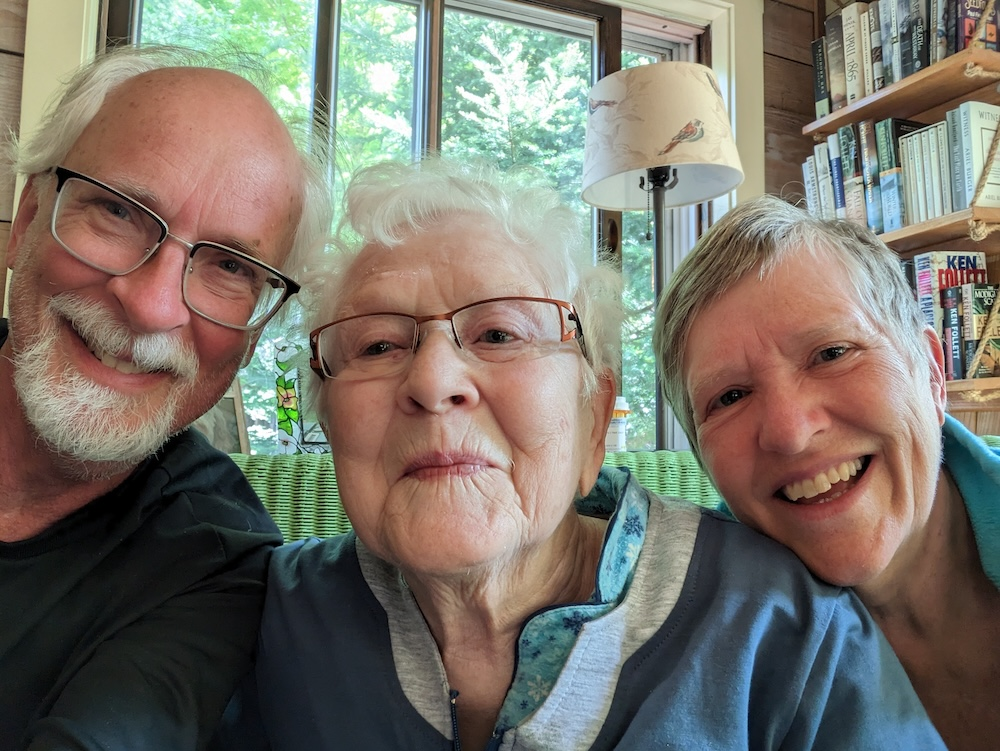
\includegraphics[width=2.14583in,height=\textheight]{AuthorPhoto.jpg}

Mark Niemann-Ross writes about whatever he damn well chooses. Mostly
science fiction, sometimes programming in R, often about tinkering with
Raspberry Pi (the single board computer, not the pastry).

He lives in Portland, Oregon, paddles boats, and gives compliments to
strangers.

\section*{Learn More about My Favorite
Mother-In-Law}\label{learn-more-about-my-favorite-mother-in-law}
\addcontentsline{toc}{section}{Learn More about My Favorite
Mother-In-Law}

\markright{Learn More about My Favorite Mother-In-Law}

There's a lot happening in the world of this book. Find out more at this
website:


\includegraphics[width=2.84375in,height=\textheight]{images/qr fave mother in law.png}

\href{http://niemannross.com/link/morefavemil}{More about my Favorite
Mother-In-Law}



\end{document}
